% Document class, language and encoding setup
\documentclass[a4paper,twoside,12pt,english]{report}
\usepackage[english]{babel}
\usepackage[utf8]{inputenc}
\usepackage[T1]{fontenc}
% Fixing the font issue
\usepackage{ae,aecompl}

%All empty pages have no page style
\usepackage{emptypage}

% Color package
\PassOptionsToPackage{dvipsnames}{xcolor}
	\RequirePackage{xcolor} % [dvipsnames] 
	
% Allows page-links in pdf file
\usepackage{hyperref}
\hypersetup{
% Uncomment the line below to remove all links (to references, figures, tables, etc)
%draft, 
%colorlinks=true, linktocpage=true, pdfstartpage=3, pdfstartview=FitV,
% Uncomment the line below if you want to have black links (e.g. for printing black and white)
colorlinks=true, linktocpage=true, pdfborder={0 0 0}, 
pdfstartpage=3, pdfstartview=FitV, hypertexnames=true, pdfhighlight=/O, 
breaklinks=true, pdfpagemode=UseNone, pageanchor=true, pdfpagemode=UseOutlines, plainpages=false,
bookmarksnumbered, bookmarksopen=true, bookmarksopenlevel=1,
urlcolor=Black, linkcolor=Black, citecolor=Black,
%------------------------------------------------
% PDF file meta-information
%pdftitle={\myTitle},
%pdfauthor={\textcopyright\ \myName, \myUni, \myFaculty},
%pdfsubject={},
%pdfkeywords={},
%pdfcreator={pdfLaTeX},
%pdfproducer={LaTeX with hyperref and classicthesis}
%------------------------------------------------
}

% Todo notes package and commands
\usepackage[colorinlistoftodos]{todonotes}

% Allows commands to emit a space "at the end"
\usepackage{xspace}

% Listings setup
\usepackage{listings}

% Algorithm2e
\usepackage[lined,boxed,commentsnumbered,linesnumbered]{algorithm2e}

% Graphics setup
\usepackage{graphicx}
\graphicspath{{./graphics/}}

\usepackage{tikz}
\usetikzlibrary{arrows}

\usepackage{amsmath}
\usepackage{amssymb}

% Clever references
\usepackage{cleveref}

% Named references
\usepackage{nameref}

% Bibliography
\usepackage[square,numbers]{natbib}
\bibliographystyle{unsrtnat}

% Force position [H]
\usepackage{float}

\usepackage{verbatim}

% Additional commands
\newcommand{\namedtodo}[5]
{
  \ifthenelse{\equal{#1}{}}
  {
    \todo[backgroundcolor=#4,caption=
    {\textbf{#3: } #2}
    ,inline]
    {\color{#5}\textbf{#3: }#2}
  }
  {
    \todo[backgroundcolor=#4,caption=
    {\textbf{#3: } #1}
    ,inline]
    {\color{#5}\textbf{#3: }#2}
  }
}
\newcommand{\mikkel}[2][]{\namedtodo{#1}{#2}{Mikkel}{blue!80}{white}}
\newcommand{\stefan}[2][]{\namedtodo{#1}{#2}{Stefan M}{orange}{black}}
\newcommand{\mikael}[2][]{\namedtodo{#1}{#2}{Mikael}{green}{black}}
\newcommand{\bruno}[2][]{\namedtodo{#1}{#2}{Bruno}{black!10!red!90}{white}}
\newcommand{\alexander}[2][]{\namedtodo{#1}{#2}{Alexander}{black!10!yellow!90}{black}}
% Her er en liste over navnene på de forskellige styles
% C#: csharp
% F#: fsharp

% 
% Listings kan refereres vha. \cref{}
\crefname{listing}{code example}{code example}
\Crefname{listing}{Code example}{code examples}
% 

%Algoritmer i cref
\crefname{algocf}{algorithm}{algorithm}
\Crefname{algocf}{Algorithm}{Algorithms}
%Algoritmelinjer i cref
\crefalias{AlgoLine}{line}%

\makeatletter
\let\cref@old@stepcounter\stepcounter
\def\stepcounter#1{%
  \cref@old@stepcounter{#1}%
  \cref@constructprefix{#1}{\cref@result}%
  \@ifundefined{cref@#1@alias}%
    {\def\@tempa{#1}}%
    {\def\@tempa{\csname cref@#1@alias\endcsname}}%
  \protected@edef\cref@currentlabel{%
    [\@tempa][\arabic{#1}][\cref@result]%
    \csname p@#1\endcsname\csname the#1\endcsname}}
\makeatother
%

% Angivelse af navn på listings
\renewcommand\lstlistingname{Code example}
\renewcommand\lstlistlistingname{Code example}

\lstdefinestyle{standard}
{
	frame=shadowbox,
	framesep=5pt,
	rulecolor=\color{blue!40!black},
	rulesepcolor=\color{white!93!black},
	numbers=left,
	basicstyle=\ttfamily,
	numberstyle=\tiny,
	numberfirstline=true,
	%numberblanklines=false,
	stepnumber=1,
	numbersep=9pt,	
	captionpos=b,
	escapeinside={(*}{*)},
	breaklines=true,
	tabsize=4,
	language=c
}

\lstset{style=standard}

\lstdefinestyle{c}
{
	style=standard
}

\lstdefinestyle{csmall}
{
	style=c
}

\lstdefinestyle{csharp}
{
	style=standard,
	language=[Sharp]C
}
\lstdefinestyle{csharpsmall}
{
	style=csharp
}
\lstdefinestyle{fsharp}
{
	language=[Sharp]F,
	frame=lr,
	rulecolor=\color{blue!80!black}
}
\lstdefinestyle{fsharpsmall}
{
	style=fsharp,
	basicstyle=\ttfamily\footnotesize
}


% Definitions
\newcommand{\projectname}{\textbf{{\color{orange}B}{\color{blue}i}{\color{green}k}{\color{red}e}{\color{purple}X}}}

% Superscript and subscript
\newcommand{\superscript}[1]{\ensuremath{^{\textrm{#1}}}}
\newcommand{\subscript}[1]{\ensuremath{_{\textrm{#1}}}}

% Degrees
\newcommand{\degree}{\ensuremath{^\circ}}
\newcommand{\dg}{\degree}

\newcommand{\quoter}[1]%
{
  \par
  \vspace{1.5em}
  \addtolength{\leftskip}{1.5cm}
  \addtolength{\rightskip}{1.5cm}
  \textit{#1}
  \addtolength{\leftskip}{-1.5cm}
  \addtolength{\rightskip}{-1.5cm}
  \vspace{1.5em}
  \par
}


\begin{document}

%Front page
\begin{titlepage}

\begin{center}
\newcommand{\HRule}{\rule{\linewidth}{0.5mm}}
\HRule \\[0.4cm]
\textsc{ \Huge City Bike \\[0.3cm]
	\Large Aalborg }\\[0.4cm]

\HRule \\[1cm]

\textsc{\Large SW701E14} \\[2cm]


\includegraphics[width=.75\textwidth]{logo}

\vfill
{\Large Internet Technology}
\\ ~\\
{\large 7\superscript{th} Semester, Fall 2014}

\end{center}
\end{titlepage}

\setcounter{secnumdepth}{3}

\cleardoublepage

\thispagestyle{empty}
\begin{titlepage}
\begin{nopagebreak}
{\samepage 
\begin{tabular}{r}
	\parbox{16cm}{\raisebox{11mm}{
\includegraphics[height=1.2cm]{aauLogoEn.jpg}}
	\hfill \parbox{7cm}{\begin{tabular}{l}
		{\small \textbf{Department of Computer Science}}\\
		{\small Selma Lagerløfs Vej 300} \\
		{\small 9220 Aalborg Ø} \\
		{\small Phone (+45) 9940 9940} \\
		{\small Fax (+45) 9940 9798} \\
		{\small \url{http://www.cs.aau.dk}}
	\end{tabular}}
	}
\end{tabular}

\begin{tabular}{cc}
	\parbox{6cm}{
	\begin{description}
		\item { \textbf{Title:}}\\
			Online Hotspot-based Predictions for Aalborg City Bike (\projectname)
    		\item { \textbf{Subject:}}\\
			\raggedright Internet Technology
		\item { \textbf{Project period:}}\\
			02-09-2014 -- 19-12-2014
 		\hspace{4cm}
		\item { \textbf{Project group:}}\\
  			sw701e14
 		\hspace{4cm}
		\item {\textbf{Participants:}}\\
			Alexander Drægert\\
			Bruno Thalmann\\
			Mikael E. Christensen\\
			Mikkel S. Larsen\\
			Stefan M. G. Micheelsen
		\item { \textbf{Supervisor:}}\\
 			Giovanni Bacci
		\item { \textbf{Printings:} 7 }
		\item { \textbf{Pages:} 54 } 
		\item { \textbf{Appendices:} 5 }
		\item { \textbf{Total pages:} 70 }
		\item { \textbf{Source code:}\\ {\small \mbox{\footnotesize\url{https://github.com/sw701e14/code/tree/d0909818e25db18b90b7111363979e8bd4c61540}}}}
	\end{description}
	\vfill } &
	\parbox{8cm}{
  	\hfill 
  	\begin{tabular}{l}
  		{ \textbf{Abstract:}} \\
  		\fbox{
  		\parbox{8cm}{\smallskip
     		{\vfill{\footnotesize The purpose of this project was to improve on the already existing \citybike system, by implementing a software solution.

In order to improve on the already existing \citybike system, it was first analyzed, identifying and defining problems to be improved upon.
Based on these problems, along with information gained from an interview with Aalborg Kommune, a solution was formed.
This solution built on-top of the current \citybike system, with the addition of GPS receivers and the removal of bike stations.

Instead of bike stations, hotspots were introduced.
These hotspots were found by using a clustering algorithm DBSCAN.
Hotspot representation was then simplified by obtaining its convex hull.

Time-homogenous Markov chains, represented as a matrix, was then introduced in order to form a model of the average bike usage.
Based on this model, predictions were made about when to expect bikes at the different hotspots.

A pseudo-realistic simulation was created in order to ensure that the implementation was successful.
The results of the tests suggest that the implementation was successful.
     		\smallskip}}}
     	}
   	\end{tabular}}
\end{tabular}
}%samepage end
\end{nopagebreak}
\end{titlepage}

\cleardoublepage

\pagenumbering{Roman}
\setcounter{page}{1}
\newcommand{\prefaceHeaderName}{Preface}
\section*{\prefaceHeaderName}
This report has been prepared by 7th semester Software Engineering students at Aalborg University, during the fall-semester of 2014.
It is expected of the reader to have a background in IT/software, due to the technical content.

References and citations are done by the use of numeric notation, e.g. \cite{civitas-archimedes}, which refers to the first item in the bibliography.

In the report, this project will henceforth be referred to as \projectname.
Whenever the report refers to 'we', it is to be understood as the members of the project group sw701e14.

Finally, we would like to thank our lecturers, and an especially big thanks to our supervisor Giovanni Bacci, for his excellent supervision throughout the semester.


%Table of contents
\pdfbookmark{\contentsname}{toc}
\setcounter{tocdepth}{1}
\tableofcontents

\cleardoublepage

\pagenumbering{arabic}

\newcommand{\introductionHeaderName}{Introduction}
\chapter*{\introductionHeaderName}
\addcontentsline{toc}{chapter}{\introductionHeaderName}
To counter the increasing energy and environmental issues, Aalborg Kommune implemented the CIVITAS-ARCHIMEDES project\cite{aalborgbycyklenbagcyklen}. As part of this project, city bikes were made publicly available for everyday use.
In order to maximize the number of users, the usage was cheap and easy but the bikes were well equipped and was of good quality\cite{cykelplanlaegning}.
To use a bike all you need to do is to place a 20DKK coin into a bike lock. When your ride is over and you lock the bike at the station, you will get your 20DKK back.

\chapter{Analysis}
\section{\citybike}\label{aalborg_bycyklen}
\citybike is a communal bike service and therefore available to anyone living in or visiting the city of Aalborg.
The service is available from the 1st of May until the end of October \cite{aalborgbycyklenbagcyklen}.

\noindent The service consists of:
\begin{itemize}
\item 200 bikes (140 active) and 
\item 21 bike stations, with room for 170 bikes in total.
\end{itemize}
Each bike is provided with a lock, that enables locking a bike to a station (similar to shopping cart systems).
The bike is unlocked by depositing a coin (20 DKK) into the lock, after which it the bike is freely available for the user.
By returning the bike to a station, and re-applying the lock at a free stand, the deposited coin is returned.

\paragraph{Missing and broken bikes} are reported through a form on the \citybike website: \url{http://www.aalborgbycyklen.dk/}.

\paragraph{The general utilization of the service} can be summarized as follows:
\begin{enumerate}
\item A user unlocks a bike at a station, by inserting 20 DKK into a locked bike.
\item The user can freely use the bike around the city.
\item The user can return the bike at any station by locking the bike.
\end{enumerate}

\subsection{Problems in the current system} \label{aalborg_bycyklen:challenges}
This section will consider the challenges associated with \citybike.
The challenges described are devised from our own experience and perspective, as there is no target group according to the domain experts (Aalborg Kommune).

%http://nordjyske.dk/nyheder/bycykler-ude-af-drift/e7a38ecd-3b1d-4290-8d2f-0f0e1a5d0fa6/4/1513
\paragraph{Bikes left outside stations}
The low deposit fee enables users to leave bikes, away from stations, without consequence other than the limited loss of 20 DKK.
It is possible to ride straight to another destination, outside a station, and leave the bike there.
The problem with this is that when someone else needs a bike, they might not be able to find one at a station, and without the possibility of knowing where they might be, outside of the stations.
Additionally, \citybike has to find the unused bikes outside stations, collect them, and return them to the stations.

\paragraph{Too few stations}
A ride is supposed to start and end at a station.
This, however, can be a problem when the user's actual start or destination is not close to a station.
Strictly speaking this shouldn't be possible, as it is not allowed to park a bike outside a station.
Practically speaking it is possible to do, and when done the problem as described in \textbf{Bikes left outside stations} emerges.

\paragraph{Making short stops}
The bikes can only be locked at stations.
This means that when a user, during a ride, wants to make a stop where there is no bike station, he has to leave his bike unlocked.
This entails a risk that a new user comes along and takes the bike (which now can be done without 20 DKK deposit, as it is not locked at a station), leaving the original user without a bike.
The original user then has to go to a station to acquire a new bike, hope to get lucky and find another bike nearby, or find another source of transportation from this point on.

\paragraph{No bikes at a station}
When users want to use a bike, they have to go to a station and see if there are any available bikes.
They have no way of knowing whether there is a bike at a station or not.
\mikael{For løst formuleret?}

\paragraph{No way of knowing when a bike will arrive}
If a user needs a bike at a specific time in a specific area, he can not be sure to find a bike at the location at the time.
\mikael{For løst formuleret?}

\paragraph{Broken bikes}
Aalborg Kommune does not know when a bike is in need of repair and rely solely on the users to report the whereabouts of broken bikes.
Potentially there could be bikes left outside the common-usage-area in need of repair. These bikes would be out of service for a long time.

\section{Interview with Aalborg Kommune}
The \citybike project is maintained by Aalborg Kommune.
In order to get information about \citybike, an interview was conducted with three people involved with the project.

The interview was carried out October 10th, 2014, as a semi-structured interview.
The interviewees were:
\begin{itemize}
\item Brian Høj; Responsible for the \citybike project.
\item Jesper; Member of the \citybike project.
\item Anne Mette; Member of the original team which implemented the CIVITAS-ARCHIMEDES project\cite{aalborgbycyklenbagcyklen}.
\end{itemize}

\noindent There were two overall goals of the interview:
\begin{enumerate}
\item To find out specifics about how the current system works.
\item To determine if the project members themselves already had improvements in mind.
\end{enumerate}

\subsection{Results} \label{interview:goals}
The following section is based on the Danish summary of the interview, found in \cref{interviewReferat}.

\paragraph{Overall goal}
The intentioned use of the bikes are single, short trips.
This means that the bikes are not meant to be used for longer periods of time, or to completely replace a personal bike.

\paragraph{Users and usage}
There is no target group for the usage of the bikes.
The bikes are currently not tracked so they were not able to say anything about the actual usage.
The only information they have is what they themselves observe when they walk around town and what citizens report.

\paragraph{Future plans}
The interviewees have before thought about installing GPS chips in the bikes to receive data about their traffic.
They would really like to have an overview of the bike usages and usage patterns.
Specifically, they would like some information about:
\begin{itemize}
\item What routes are travelled?
\item How long a distance has been travelled in this trip?
\item When was the bike used?
\item Who uses the bikes?
\end{itemize}

\paragraph{Rent/Booking}
It has never been the intention of the project to be able to rent or book a bike, because it would hamper the spontaneous use of the bikes.
If all the problems with booking could be solved in a reasonable manner, they would not rule out the future of such a system.

\paragraph{Missing bikes}
According to Traffic \& Roads, Aalborg Kommune\cite{cykelplanlaegning} there was a 11\% loss of bikes from 2009 to 2011 (237 to 210 bikes).
According to the interviewees there now, fall 2014, remain 200 of the original 237 bikes from summer 2009.
The interviewees saw this as such a small reduction in bikes, that missing and stolen bikes are not considered a problem.

\subsection{Conclusion}
The interview did not give much information about the users or usage of the system.
The target users are therefore considered to be anyone living in or currently situated in Aalborg.
Additionally, no concrete conclusions can be made about where the bikes are used the most.

The interviewees did have some restrictions and other wishes.
They did not like the idea of a renting/booking system, as they saw it to be too restricting.
They did, however, think it would be useful to track the bikes' users and usage, possibly via GPS.

\paragraph{Further contact}
After the interview we tried to contact Aalborg Kommune again, but despite several attempts, it was not possible to come into contact with them.

\section{Existing Systems}

Already existing systems are explored in order to draw inspiration from them.
They will also serve as guidelines to what should and shouldn't be repeated in a proposal of a new system.

There are many public bike systems around the world, mainly in bigger cities.
The systems differ a lot in both how and where bikes are acquired and how the use of the bikes is paid.
The two overall methods lie in either a rent-system or an grab-if-available-system.
The rent-systems usually have very few stations, and bikes are rented for a longer period of time (days), similar to a car rental service.
Aalborg Bycyklen is an example of a grab-if-available-system.

Chosen for comparison are two systems; Bycyklen\footnote{Translation from Danish: 'The City Bike'}, located in Copenhagen and Citi Bike NYC, located in New York City.
These systems are similar to Aalborg Bycyklen, in that the bikes are publicly available, and at many different locations.

These two systems have been chosen also because of the social similarities of the cities with respect to Aalborg.
Rent-systems will not be considered, as these are too different from the more publicly available systems.

\subsection{Copenhagen: Bycyklen}
The overall purpose of Bycyklen\cite{cph_bycyklen}\cite{cph_bycyklen_conditions} is to provide bikes for both single and repeated use.

A bike is rented at an hourly rate of 25 DKK/hour.
In exchange for a fixed subscription of 70 DKK/month, the hourly rate is reduced to 6 DKK.
In both cases, an account must be created first.
This can be done using an internet browser or the bike-mounted tablet.

To use the service the user has to log-in with an existing account.
The bike is then unlocked from the rack and the hourly charges begin.
Once the bike is no longer in use and placed in a rack again, the user is logged out and the bike is locked.

If a bike is left outside a bike station for longer than 2 hours, fees are charged (200 DKK in Copenhagen/Frederiksberg, 800 DKK outside), or if it has been in use for longer than 10 hours (500 DKK).
For short stops during a trip, the lock can be locked with an analogue lock, which is unlocked the same way as at a station, but only for the currently active user.

It is possible to reserve a bike by using their web page, which in all cases cost 10 DKK.
This will hold a bike, by locking it, up to 45 minutes before it is needed.
Half an hour before the reservation time, a text is sent to inform whether a bike was successfully held or not.
Repeated reservations are allowed.

Currently, there is a total of 20 stations and an estimated average of 15 bikes per station, giving a total of approximately 300 bikes.
The bike itself is electrically powered and equipped with GPS and a handlebar-mounted tablet.
The tablet is used for registration and signing in/out.
Additionally the tablet, with use of the GPS, can provide navigational guidance.

\subsection{New York City: Citi Bike NYC}
Citi Bike NYC\cite{nyc_citibike} is a system which makes available bikes for single use, but many times.

Unlike most other systems, you do not rent a single bike.
There are three methods of renting bikes:

\begin{itemize}
\item 24-hour pass: \$9.95
\item 7-day pass: \$25
\item Annual membership: \$95
\end{itemize}

With the 24-hour and 7-day passes, you can use a bike for an interval of 30 minutes at a time.
With annual membership this interval is extended to 45 minutes.
However, after each interval, you can just acquire another bike.
If you do not return the bike after the interval, overcharge fees occur.

In order to acquire a bike with a pass, a payment is made with a credit-card at a bike-station, which provides a single-use code.
This code is entered on the bike itself, which is equipped with a tablet solely for this purpose, which will unlock the bike from the bike-rack.
Along with the pass fee, a \$101 security hold is placed.
When a bike is returned, and another bike is to be acquired, the credit-card must be used again.
The credit-card will not be charged again if a pass is already active, instead a new code is provided.
For annual memberships a key is used to unlock bikes and no interaction with the bike-station is needed.

The exact number of bikes and stations is unknown.
The official website states that there are ''100s of stations'' and ''1000s of bikes''\cite{nyc_citibike}.
The bikes are very simple, with no motor or GPS, and the tablet in front is only used for unlocking bikes with either pass-code or membership-key.

\subsection{Evaluation}
Based on the problems described in \cref{aalborg_bycyklen:challenges}, the existing systems will be evaluated in regards to whether they solve all or some of these problems.

\paragraph{Bikes disappear}
In Bycyklen, this is partially, indirectly solved by the hourly charges until the bike is returned, along with the additional fees if the bike is immobile for 2 hours or used for more than 10 hours.
Presumably, the GPS in the bikes can also be used to locating misplaced bikes (This is based on the fact that users agree to let Bycyklen collect anonymous data about start/end destination, and route usage).

In Citibike NYC overcharge fees are continuously charged, after exceeding the allowed half hour trip, until it is returned to a bike station.
Nothing can be found about whether this goes on forever or not.

\paragraph{Flexibility}
Bycyklen provides an analogue lock, for short stops (2 hours) during use.
However, when done using a bike it must be returned to a station.

In Citi Bike NYC, the multitude of stations and the placement throughout the city should make sure that there is always a station close-by, no matter where you want to end your trip, including shorter stops.

\paragraph{Reliability}
Both Bycyklen and Citibike NYC have web apps with a map showing stations, along with an indication of how many bikes are available at the different stations.
Citibike NYC also has native mobile apps, while Bycyklen only has the web app.

The reservation system of Bycyklen cannot ensure that a bike will be available, as it will only attempt to lock a bike 45 minutes before the reservation time if a bike is available.

Citibike NYC has no reservation system, one must consult an app for available bikes at stations, but the multitude of  available bikes should ensure that there's always a bike, and the multitude of stations should ensure that you will not have to go far if no bike was at the first visited station.

\paragraph{Broken bikes}
Before using a Bycyklen bike, all faults on the bike must be reported, or else the user can be charged for faults found by the next user.
Faults must also be reported during use, and if a fault hinters a trip, a refund can be made.

Using the mounted tablet on a Citibike NYC bike, one can report faults/damages by pressing a wrench-icon button.
If faults are found during use, the bike is simply returned at a station and the aforementioned button is pressed.

\subsection{Conclusion}
Both systems do well in handling all the problems described in \cref{aalborg_bycyklen:challenges}

They do however not suit the goals of the projects stated by Aalborg Kommune in \cref{interview:goals}

Additionally they are both costly systems, and cannot be easily built on top of the current Aalborg Bycyklen system because they require a lot of changes to the bikes and stations to accommodate for the locking and renting mechanics of the two systems.

Another problem is the lack of usage statistics in the current system, meaning that it is not easy to find out where to put stations (which both existing systems require).
In case too few stations are set up, or are poorly placed, it could affect both the flexibility and the reliability problem.


\section{Problem statement}
This section contains the main problem for this project and the form of solution required.

\subsection{Analysis Summary}
The analysis was based on the initial problem: \textit{How can the current \citybike system be improved, in order to make it more usable?}.
From the analysis, it was found that the current \citybike has several problems, limiting the overall usability (as described in \cref{aalborg_bycyklen:challenges}).

The problems identified were:
\begin{enumerate}
\item Bikes left outside stations \label{pr_stations}
\item Too few stations \label{pr_few}
\item Making short stops \label{pr_stops}
\item No bikes at station \label{pr_nobikes}
\item No way of knowing when a bike will arrive \label{pr_arrive}
\item Broken bikes \label{pr_broken}
\end{enumerate}

Additionally, certain limitations and requests were made by Aalborg Kommune, collected through the interview:

\begin{enumerate}
\item No renting/booking system
\item No specific target user group
\item Statistics about usage
\item Short period usage
\end{enumerate}

\subsection{Scope}
Due to the limited time and project members, certain restrictions will be set, as to remove focus on certain problems.

\paragraph{Making short stops} will be completely overlooked in this project, as any solution to this problem would require some added locking mechanisms, which would conflict with the limitations set by Aalborg Kommune.

\paragraph{Statistics about usage} is something Aalborg Kommune also requested.
This, however, is deemed too far from the initial problem, as we won't be able to get any significant data without testing it on the actual bikes.

\subsection{Solution} \label{prob_statement:solution}
We have chosen the solution with the same bikes as the current system, with the addition of a GPS chip on each individual bike, and completely removing the stations and bike locks.
This is due to the restrictions set by Aalborg Kommune, requesting a simple system, in order to accommodate the unspecified target user group.

\paragraph{GPS and hotspots}
The greatest changes to the current system is the addition of the GPS and the introduction of hotspots.
Hotspots will serve as informal stations; areas of the map where bikes are often parked.
By combining these two things, we want to improve on the problems with the current system.

\subparagraph{\ref{pr_stations}: Bikes left outside stations} is handled by GPS, as bikes and their exact location now can be found, no matter if it is at a hotspot or not.

\subparagraph{\ref{pr_few}: Too few stations} is automatically handled by the generation of hotspots.
Whenever an area is a popular place to be going from/to, a hotspot should emerge and reflect this.

\subparagraph{\ref{pr_stops}: Making short stops} was deemed out of scope.

\subparagraph{\ref{pr_nobikes}: No bikes at station} is handled by locating the exact location of an available bike, or looking up nearby hotspots.

\subparagraph{\ref{pr_arrive}: No way of knowing when a bike will arrive} will be handled by modeling bike behavior and predicting when a bike will be available at certain hotspot(s).

\subparagraph{\ref{pr_broken}: Broken bikes} will not be directly handled, but it is possible to infer from looking at bike locations and detecting when a bike has been immobile for a very long time, which could indicate that it either is too far away for anyone to pick it up, or broken.

\paragraph{Software}
A software solution is then to be developed, consisting of 3 main software components, and a shared database.
The structure of the solution can be seen in \Cref{fig:solution_structure}.

\begin{figure}[h]
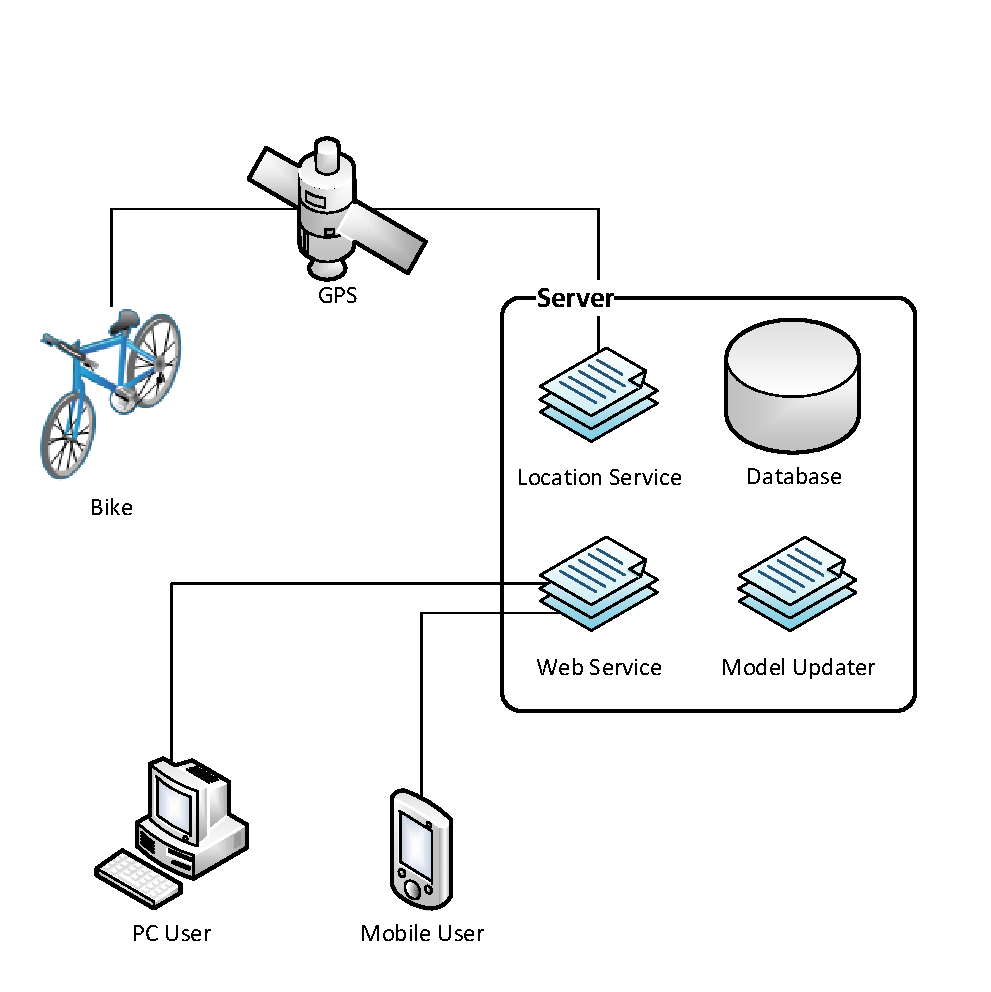
\includegraphics[width=\textwidth, trim={0cm 1cm 2cm 1.5cm}]{our_solution.pdf}
\caption{The overall structure of our solution}
\label{fig:solution_structure}
\end{figure}

The \textit{Location Service} continuously updates the locations of the bikes.
The \textit{Model Updater} uses the stored location data to generate a model used for predictions.
The \textit{Web Service} makes an API available, in order to make platform implementations to make the data available as specified in the requirements.
A web service was chosen as to make the system as available as possible, due to the unspecific target user group.

\subsection{New problems}
In order to develop this new system,\alexander{Is it really a `new system'?} with the addition of GPS and hotspots, new problems emerge.
The following chapters will focus on the problems:
\begin{itemize}
\item How to define and find hotspots?
\item How to model the usage and use this for predictions?
\item How to make this data available through a web service?
\end{itemize}\alexander{Add `How to simulate realistic data'?}

\chapter{Predicting Behaviour}
\section{Modeling Behavior}\label{modelbehavior}
As the purpose of \projectname{} is to be able to predict the movement of bikes at a given time (see \Cref{problem_statement}), it must be able to answer questions such as: 

\begin{itemize}
\item How much time will it take before a bike will be in my vicinity?
\end{itemize}

The location of the bikes are abstracted by creating hotspots, as described in \Cref{hotspots}.
In actuality, the location of bikes is modeled to be more complex as will be further explored in \Cref{markov:modeling}.
However the theory and methods described in the following sections apply regardless.

By abstracting the locations to be hotspots the above question can be rephrased as: 

\begin{itemize}
\item How much time will it take before a bike will be \emph{in a given hotspot}?
\end{itemize}


To answer this question we need to model the behavior of an \emph{average} bike.
In other words, we need to provide a formal description of the movement of a single bike representing the movement, on average, of all bikes.

\subsection{Abstraction Model}
As the system is based on anonymous usage no user sensitive information is collected.
Because of this some uncertainty is expected in the model, as all bikes (and thus all users) are modeled as a single \textit{average bike}.
Modeling the movement of all bikes will be done by modeling the movement of this average bike as a stochastic process \cite{stochastic}.

We must also consider that our model will be working on discrete-time location data.
The GPS units that the bikes will be equipped with will only report the location of a bike at a \textit{fixed} interval.
Additionally the accuracy of each of these measurements can be low, resulting in even more imprecision.
As we are modeling the average bike, we can represent the state of the process as the location of the bike.
In order to reduce the number of locations to a sensible number we will use the generated hotspots instead.
Using this definition we can describe the movement of the bike as an infinite route $h_1, h_2, h_3, \dots$ where $h_i \in H \mid i \in \mathbb{N}$ and $H$ is the set of hotspots in the system.

Using this representation of the average bike we see that the average bike must move from one hotspot $h_i$ to another $h_{i+1}$ in one \emph{timestep}.
Note that it could be that $h_i = h_{i+1}$, meaning that the bike has moved to the same hotspot as it departed from.
This is also used to indicate that the bike has not moved.
In \Cref{markov:modeling} we will describe the modeling of the average city bike in greater detail.

Taking all of the above into account it is reasonable to suggest the abstraction model for the behavior of the average city bike, to be a discrete-time Markov chain where the states are used to represent hotspots.

\subsection{Discrete-Time Markov Chains}\label{markov}
The state of a discrete-time Markov chain model changes in a process at discrete time intervals.
It can be viewed as a sequence (chain) of random variables $X_1, X_2, X_3, \dots$ where each such variable is a function $X_i:S \rightarrow x$.
Here $S$ is a countable set of states representing the possible states (hotspots) in the process described by the Markov chain and $x$ is a \textit{random} state from $S$.
The subscript describes the time associated with each of the variables.
Thus $X_i$ represents the possible states of the process at time $i$.
This notation allows us to establish a timespan as each step refers to a fixed interval.

This randomness will be biased towards certain states given its current state (and possibly time) resulting in a set of probabilities for each state given a random variable.
Let $\mathbb{P}(X_i = x)$ be the probability of $X_i$ being in state $x$.
The above will then allow us to express the probability of moving to a state $y$ given the path we have traversed.
In other words, knowing what state we are in and how we got to it allows us to determine the probability of the next state being $y$:

$$\mathbb{P}(X_{n+1} = y \mid X_1 = x_1, X_2 = x_2, \dots X_n = x)$$

\paragraph{Markov property}\label{markov:property}
For the sequence to describe a Markov chain it must additionally have the Markov property.
The Markov property states that for any state $x$ we can determine the probability of the next state being $y$ without any knowledge of the path that led to $x$.
We can formalize this as:

\begin{align}\label{markov:eq:markov_prob}
\mathbb{P}(&X_{n+1} = y \mid X_1 = x_1, X_2 = x_2, \dots X_n = x)\nonumber\\
= \mathbb{P}(&X_{n+1} = y \mid X_n = x)
\end{align}

\paragraph{Time-homogeneous Markov chains}
In an effort to simplify the problem of predicting the behavior of the average bike we will be using time-homogeneous Markov chains.
A Time-homogeneous Markov chain can also be thought of as a time-independent chain.
In other words, predicting the next state of the chain can be done without knowledge of the time:
\begin{equation}
\mathbb{P}(X_{m+1} = y \mid X_m = x) = \mathbb{P}(X_{n+1} = y \mid X_n = x)
\end{equation}

Time-homogeneous Markov chains provides us with a much simpler method of modeling the average bike.
A time-homogeneous Markov chain is very simple to represent (as is described below) and easy to use when predicting the state of the average bike multiple steps into the future.
For these reasons we have chosen to simplify our Markov chain models.

This simplification will mean that we are unable to determine a difference in behavior at different times in the process.
Thus we cannot, using a single model, represent different behaviors of the average bike in the morning/afternoon or in different days of the week.
To allow for this distinction multiple models could be generated, representing different datasets.
The system would then simply select the model that corresponds to the current time-of-day/day-of-week.

\paragraph{Mathematical representation}\label{markov:math}
From the above definitions we have that a Markov chain $\mathcal{M}$ can be described as a function $\tau_M:S\times S \rightarrow [0;1]$ such that $\tau_M(x, y) = \mathbb{P}(X_{n + 1} = y \mid X_n = x)$.
As the chain is independent of time we can represent it using a single matrix containing all its transitional probabilities.
Below is a generic representation of such a matrix:

\begin{equation}\label{markov:matrix}
\begin{bmatrix}
\tau_M(s_0, s_0) & \tau_M(s_0, s_1) & \cdots & \tau_M(s_0, s_n)\\
\tau_M(s_1, s_0) & \tau_M(s_1, s_1) & \cdots & \tau_M(s_1, s_n)\\
\vdots & \vdots & \ddots & \vdots\\
\tau_M(s_n, s_0) & \tau_M(s_n, s_1) & \cdots & \tau_M(s_n, s_n)
\end{bmatrix}
\end{equation}

This is a simple representation that allows us to predict probabilities multiple steps into the future by applying the same matrix to some initial probability distribution multiple times.

\paragraph{Visual representation}
Markov chains are typically represented using a DAG\footnote{Directed Acyclic Graph} with weight on its edges.
In such a graph nodes represent states and the weight of edges represent the probability of transitioning between two states.
This is a direct mapping of the matrix described above.

In \Cref{markov:model:simple} we give an example of a Markov chain that models an average city bike traveling back and forth between two hotspots $\{H_1, H_2\}$.
From the weights on the diagram edges we can read the time-homogeneous probability of moving from one state to another (or staying in the same state).
For instance, a Markov chain currently in $H_1$ has probability $0.7$ of transitioning to $H_1$ (staying) and probability $0.3$ of transitioning to $H_2$.

In the diagram there are no edges with weight zero.
Any such edges would represent transitions with zero probability (\textit{``impossible``} transitions).
Had there been edges with weight zero, they could have been removed to simplify the graph.
This also means that any \textit{missing} edge between two states $s_1$ and $s_2$ implies that $\tau(s_1, s_2) = 0$.
Examples of this can be seen in \Cref{markov:model:complex} where states $D_1$ and $D_2$ are not connected.

\subsection{Modeling the average bike}\label{markov:modeling}
\texttt{New}\\
Throughout this section we have described the modeling of the average bike as a distribution on a set of infinite paths of hotspots.\\
\texttt{Old}\\
Throughout this section we have described the modeling of the average bike as an infinite path of hotspots.
\mikael{Giovanni stadig ikke tilfreds med den her.}
\bruno{Hvad er han ikke tilfreds med?}
\alexander{Something about the average bike being modeled as an `infinite path of hotspots'.}
\alexander{I have given it a shot, read it and tell me what you think.}
We represent a simple example of this, using only two hotspots, in \Cref{markov:model:simple}.
\begin{figure}[H]
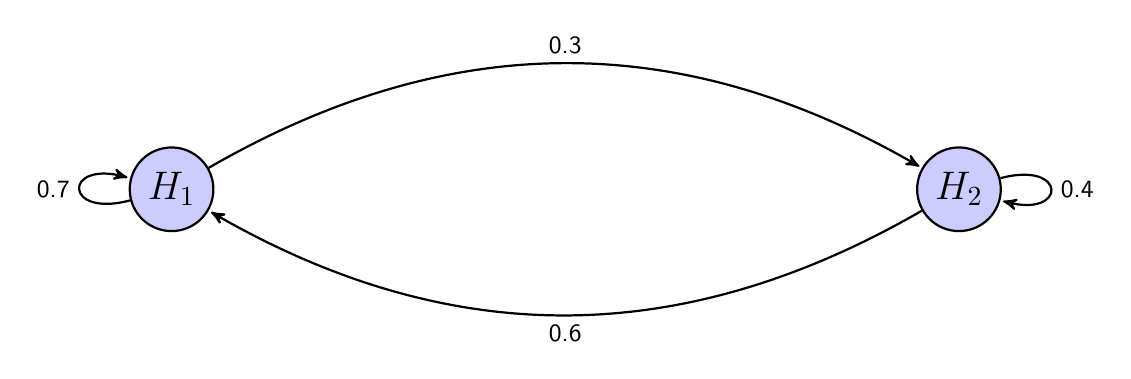
\begin{tikzpicture}[->,>=stealth',shorten >=1pt,auto,node distance=10cm,
  thick,main node/.style={circle,fill=blue!20,draw,font=\sffamily\Large\bfseries}]

  \node[main node] (1) {$H_1$};
  \node[main node] (2) [right of=1] {$H_2$};

  \path[every node/.style={font=\sffamily\small}]
    (1) edge [bend left] node {0.3} (2)
        edge [loop left] node {0.7} (1)
    (2) edge [bend left] node {0.6} (1)
        edge [loop right] node {0.4} (2);
\end{tikzpicture}
\caption{A Markov chain model of a system with two bike hotspots}
\label{markov:model:simple}
\end{figure}
Using this system we will be able to make predictions on the path of the bike in the system.
To do this we require an initial state for the system.
This state should represent the current (at the time of a query) location of the bikes in the system.
Using this representation we will be able to compute the probability that the bikes will be in some hotspot after a number of time steps.

\paragraph{Insufficient states}
As we are looking to use the Markov chains to predict whether or not a bike is available at a hotspot we must also be able to represent whether they are in use or not.
The modeling described so far only allows for a bike to be at a hotspot and thus we are not able to give a direct representation of a bike in transit.

To accommodate this restriction we introduce an additional state for each of the hotspots.
These states are called \emph{departure states} and the departure state associated with hotspot $H_i$ is denoted as $D_i$.
The simple two-hotspots model described above can then be expanded with departure states, as seen in \Cref{markov:model:complex}.

\begin{figure}[H]
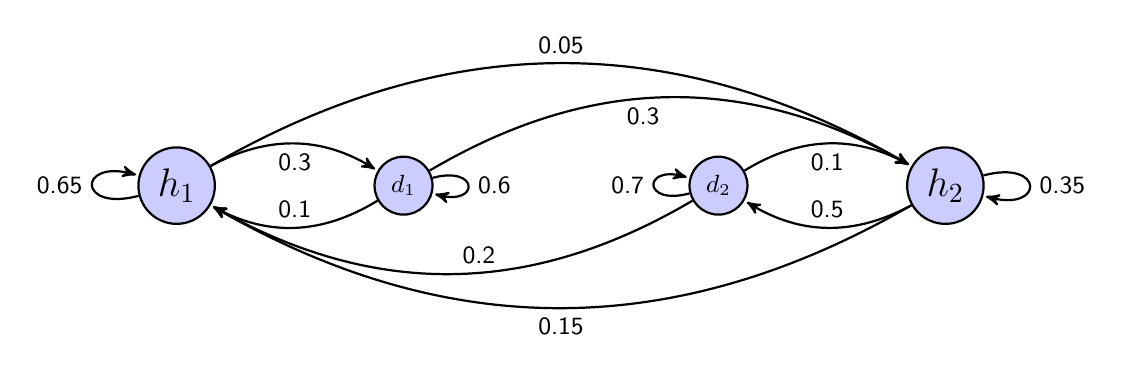
\begin{tikzpicture}[->,>=stealth',shorten >=1pt,auto,node distance=4cm,
  thick,main node/.style={circle,fill=blue!20,draw,font=\sffamily\Large\bfseries}]

  \node[main node] (B1) {$h_1$};
  \node[main node,font=\sffamily\small] (D1) [right = 2cm of B1] {$d_1$};
  \node[main node,font=\sffamily\small] (D2) [right of=D1] {$d_2$};
  \node[main node] (B2) [right = 2cm of D2] {$h_2$};

  \path[every node/.style={font=\sffamily\small}]
    (B1) edge [bend left] node {0.05} (B2)
         edge [loop left] node {0.65} (B1)
         edge [bend left] node[below] {0.3} (D1)
    (B2) edge [bend left] node {0.15} (B1)
         edge [loop right] node {0.35} (B2)
         edge [bend left] node[above] {0.5} (D2)
    (D1) edge [bend left] node[above] {0.1} (B1)
         edge [loop right] node {0.6} (D1)
         edge [bend left] node[below left] {0.3} (B2)
    (D2) edge [bend left] node[below] {0.1} (B2)
         edge [loop left] node {0.7} (D2)
         edge [bend left] node[above right] {0.2} (B1);
\end{tikzpicture}
\caption{A Markov chain model with two hotspots and departure states}
\label{markov:model:complex}
\end{figure}

% VISUALIZE
% http://setosa.io/blog/2014/07/26/markov-chains/index.html
%[[0.65,0.30,0.05,0.00],
%[0.10,0.60,0.30,0.00],
%[0.15,0.00,0.50,0.35],
%[0.20,0.00,0.10,0.70]
%]

These states allow us to represent bikes that are not currently located at a hotspot.
Note that in this model some transitions are not possible.
These are $D_i \rightarrow D_j$ and $H_i \rightarrow D_j $ for $i \neq j$ transitions.
This models the fact that a bike must transit through $H_j$ before it can arrive at its departure state $D_j$.

This model allows us to initialize a Markov chain using some initial state representing the current (the time of a query) location of the bikes and then predict where the bikes will be located after a number of time steps.
From this prediction it is then possible to predict how many bikes should be available at a given hotspot in a given timespan according to our model.

\paragraph{Ordered matrix}
To ensure that the various parts of this section, as well as the implementation, works consistently we introduce a set ordering of states in the matrix.
In this representation of the matrix $(x, y)$ is used to denote $\tau_M(x, y)$.
This is done solely to simplify the matrix.

\begin{equation}\label{markov:matrix-ordered}
\begin{bmatrix}
(h_0, h_0) & (h_0, d_0) &
(h_0, h_1) & (h_0, d_1) &
\cdots &
(h_0, h_n) & (h_0, d_n)\\

(d_0, h_0) & (d_0, d_0) &
(d_0, h_1) & (d_0, d_1) &
\cdots &
(d_0, h_n) & (d_0, d_n)\\


(h_1, h_0) & (h_1, d_0) &
(h_1, h_1) & (h_1, d_1) &
\cdots &
(h_1, h_n) & (h_1, d_n)\\

(d_1, h_0) & (d_1, d_0) &
(d_1, h_1) & (d_1, d_1) &
\cdots &
(d_1, h_n) & (d_1, d_n)\\


\vdots & \vdots & \vdots & \vdots & \ddots & \vdots & \vdots\\


(h_n, h_0) & (h_n, d_0) &
(h_n, h_1) & (h_n, d_1) &
\cdots &
(h_n, h_n) & (h_n, d_n)\\

(d_n, h_0) & (d_n, d_0) &
(d_n, h_1) & (d_n, d_1) &
\cdots &
(d_n, h_n) & (d_n, d_n)
\end{bmatrix}
\end{equation}

\section{Clustering}\label{clustering}
In order to find the hotspot(s) defined in \Cref{hotspot}, we considered different clustering techniques.
This section will describe the concepts of clustering as well as the possible algorithms.
This section is based on \citet{pang2006introduction}.

\subsection{Cluster Analysis}
Cluster analysis is a technique used to group data objects based only on the information the data itself contains.
The requirement for membership in a certain cluster is often vague, as several acceptable clusterings can be made on the same dataset.
An example of this can be seen in \Cref{clusterings}, where the same dataset has been clustered in three radically different ways, even though all three could be regarded as correct, depending on the purpose of the clustering.
The clustering therefore depends on the dataset and its purpose.

\begin{figure}[H]
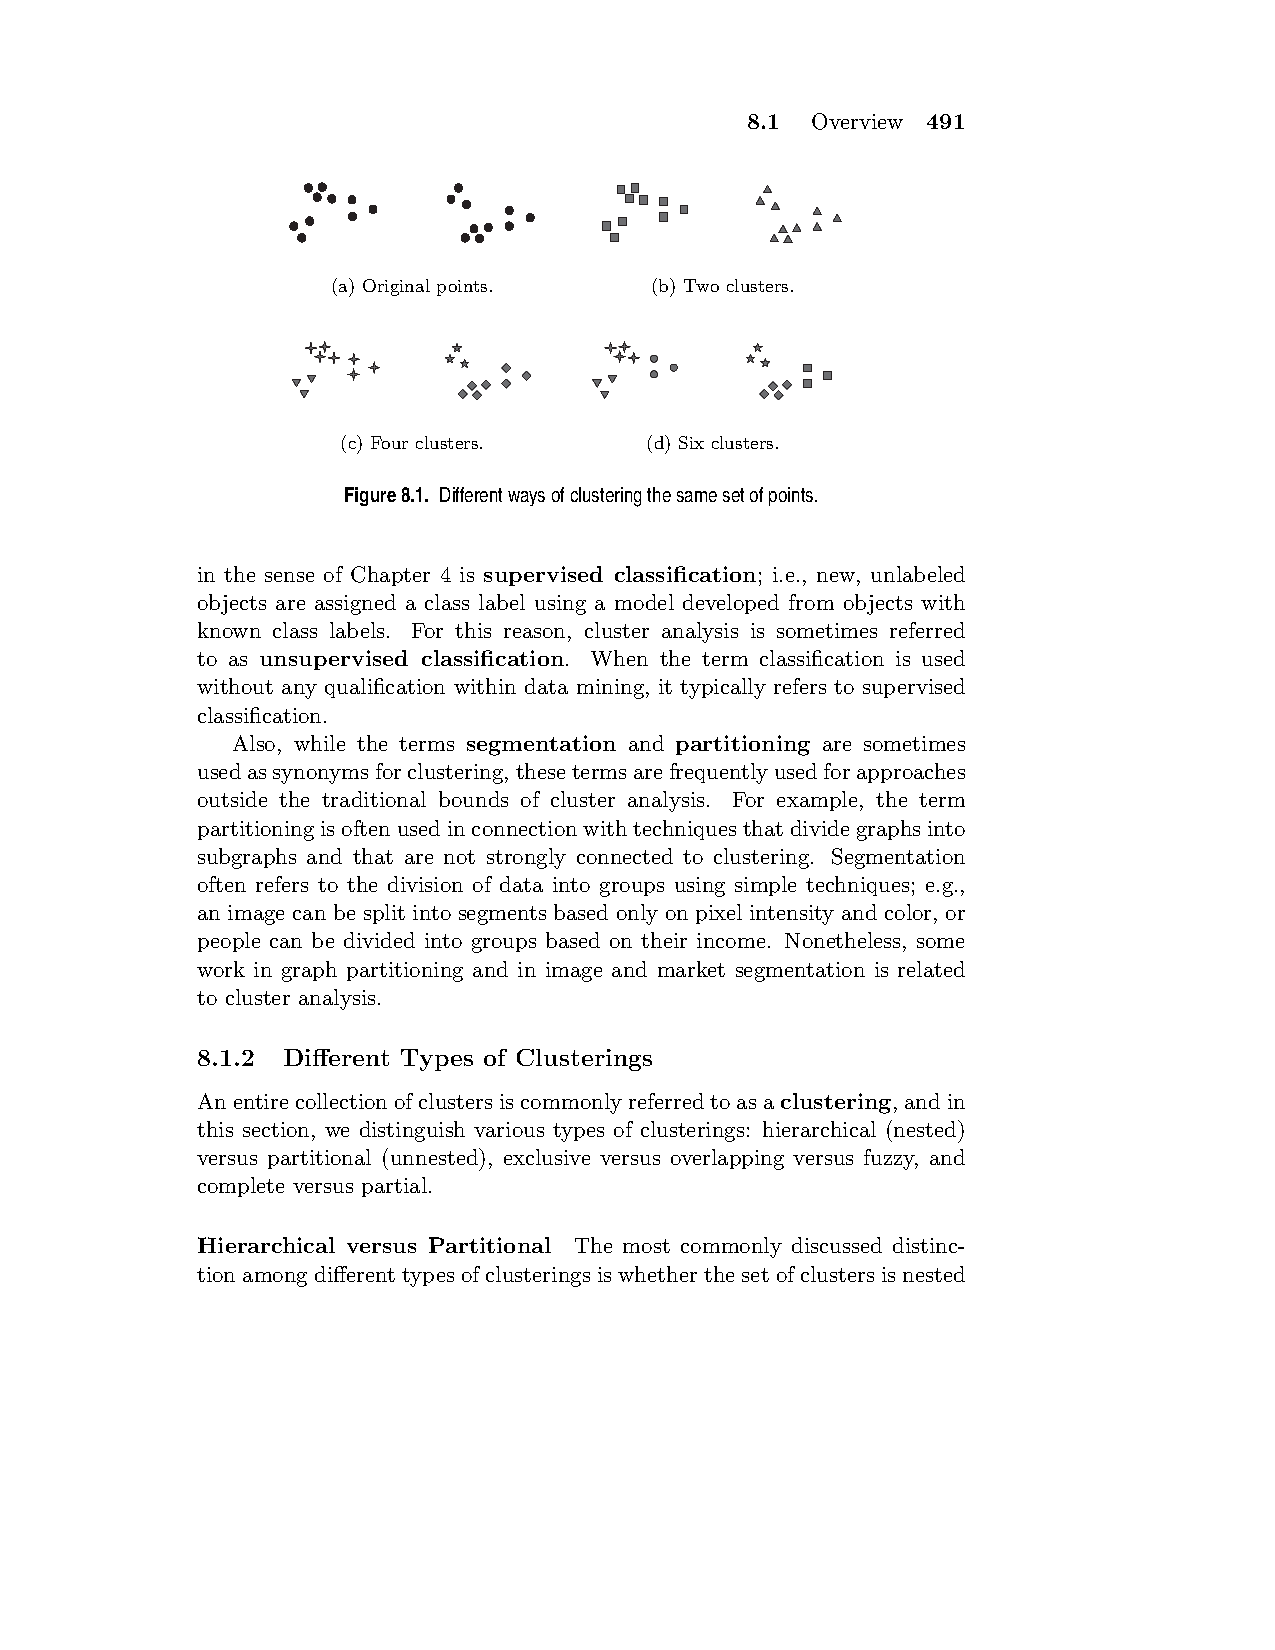
\includegraphics[trim= 3.1cm 19.91cm 5cm 2.5cm, clip=true]{graphics/different_clusters}
\centering
\caption{Different clusterings on the same dataset. From \citet{pang2006introduction}.}
\label{clusterings}
\end{figure}

\subsection{Types of clusterings}

A clustering is a collection of clusters.
This section will introduce the terminology used to describe clusterings. 

\paragraph{Hierarchical versus partitional}
A \textit{partitional clustering} is a division of data into pairwise disjoint subsets, where each object belongs to exactly one subset.
If clusters are allowed to have subclusters, the clustering is said to be \textit{hierarchical}.
A hierarchical clustering is represented as a set of nested clusters organized as a tree, where each node is the union of its children.

\paragraph{Exclusive, overlapping and fuzzy clusterings}

A clustering is \textit{exclusive} if an object is assigned to exactly one cluster.
If an object can belong to more than one group, the clustering is said to be \textit{overlapping}.
If a weight is used to describe the membership of sets, the clustering is said to be \textit{fuzzy}.

\paragraph{Complete versus partial}

A \textit{complete} clustering has every object assigned to a cluster, while a \textit{partial} clustering can have outliers; objects that do not belong to any cluster.

\subsection{Types of clusters}
The purpose of a cluster depends on the kind of data set it is applied on.
In this section, the different notions of a cluster will be presented.

\paragraph{Well separated}
A cluster is a set of objects, where the objects that are similar are grouped in a cluster. 
Sometimes a threshold is used to define a minimum similarity. 
All objects in a cluster need to be at least as similar to all other objects in the cluster, for an object to be in the cluster.

\paragraph{Prototype based}
Objects are placed in clusters based on the prototypes that define the clusters.
An object is placed in the cluster where the object is more similar to the prototype of that cluster, than to the prototype of all other clusters.

These prototypes can be either the average value of a cluster, or the most representative object of a cluster.

\paragraph{Graph based}
If the data can be represented as a graph, with the objects as nodes, clusters can be defined as connected components in the graph.

\paragraph{Density based}
A cluster is defined by the density of the data objects.
A cluster is a dense region surrounded by a low density region.

\subsection{Our data and purpose}
The data we need to cluster is GPS data from the bikes.
A bike will send a GPS location in some interval, and it will be saved in a database.
We expect the points to be distributed in a wide area, but clustered around places where people place the bikes.
These clusters may have different size depending on the physical properties of the places the bikes are left.

The purpose of the clustering is to find the areas where the bicycles are being used the most in order to make predictions on when a bike will arrive in those areas.
A polygon will be used as a representation of a cluster, more about that in \Cref{convex_hull}.

Based on this description we need a hierarchical, exclusive, partial and density based clustering.

Hierarchically because we want to represent the clusters as a polygon.
This would ease the task of point location.
It needs to be exclusive because we want the clusters to be separated from each other so any point on the map is either in one cluster or not in any cluster.
We want to find out where the bikes spend most of their time and therefore we want a density based partial clustering.

\subsection{Techniques}
This section will explore the techniques that exist in cluster analysis and evaluate them based on the requirements stated in the previous section.

\subsubsection{K-means}
K-means is a technique that creates a partitioning from prototypes where the prototypes are the center of the clusters.

The basic algorithm takes a number K and generates K initial center points.
Each data object is then assigned to the nearest center point.
The center points are now updated to be the center of the created clusters.
These steps are repeated until no point changes cluster or the center points do not change.

Because we do not have a way of finding $ k $ before running the algorithm, this approach is not applicable to our problem.

\subsubsection{Hierarchical Clustering}
Hierarchical clustering arranges the points in a hierarchy depending on the distance between points.
Hierarchical clustering can be performed either by starting at the top of the tree or at the bottom.
\textit{Agglomerative hierarchical clustering} starts by considering all points as being in an individual cluster and generating the hierarchy by merging the closest clusters. 
\textit{Divisive hierarchical clustering} starts by considering all points as being in a single cluster and then continues by splitting the clusters at each step.

We have no need for a hierarchical division of our clusters, and this algorithm is therefor not appropriate for our use.

\subsubsection{DBSCAN}\label{clustering:DBSCAN}
DBSCAN in a density based clustering algorithm that locates regions of high density that are separated by regions of low density.

\paragraph{Center based point density}
There exists different methods of determining density in a set of data points.
One approach is to use a point as a center and calculate the number of points that are within a certain radius of the point.
Using this measure it can be classified whether a point is placed in a dense region (a core point),at the edge of a dense region (a border point) or is in a region with sparse density (a noise point).
The exact definition of the three types of points are as follows\cite{pang2006introduction}:
\\
\\
\noindent
\textbf{Core point} These points have at least $ MinPts $ points in a radius of $ eps $ from it.
Here $ MinPts $ is the number of points in the vicinity of a point regarded as dense by the user, and $ eps $ is the radius to look for these points.

\noindent
\textbf{Border points} A point that is not a core point, but is in the neighborhood of a core point. 
One point can be a border point to several core points.

\noindent
\textbf{Noise point} Any point that is neither a core point or a border point. 

\begin{figure}
\fbox{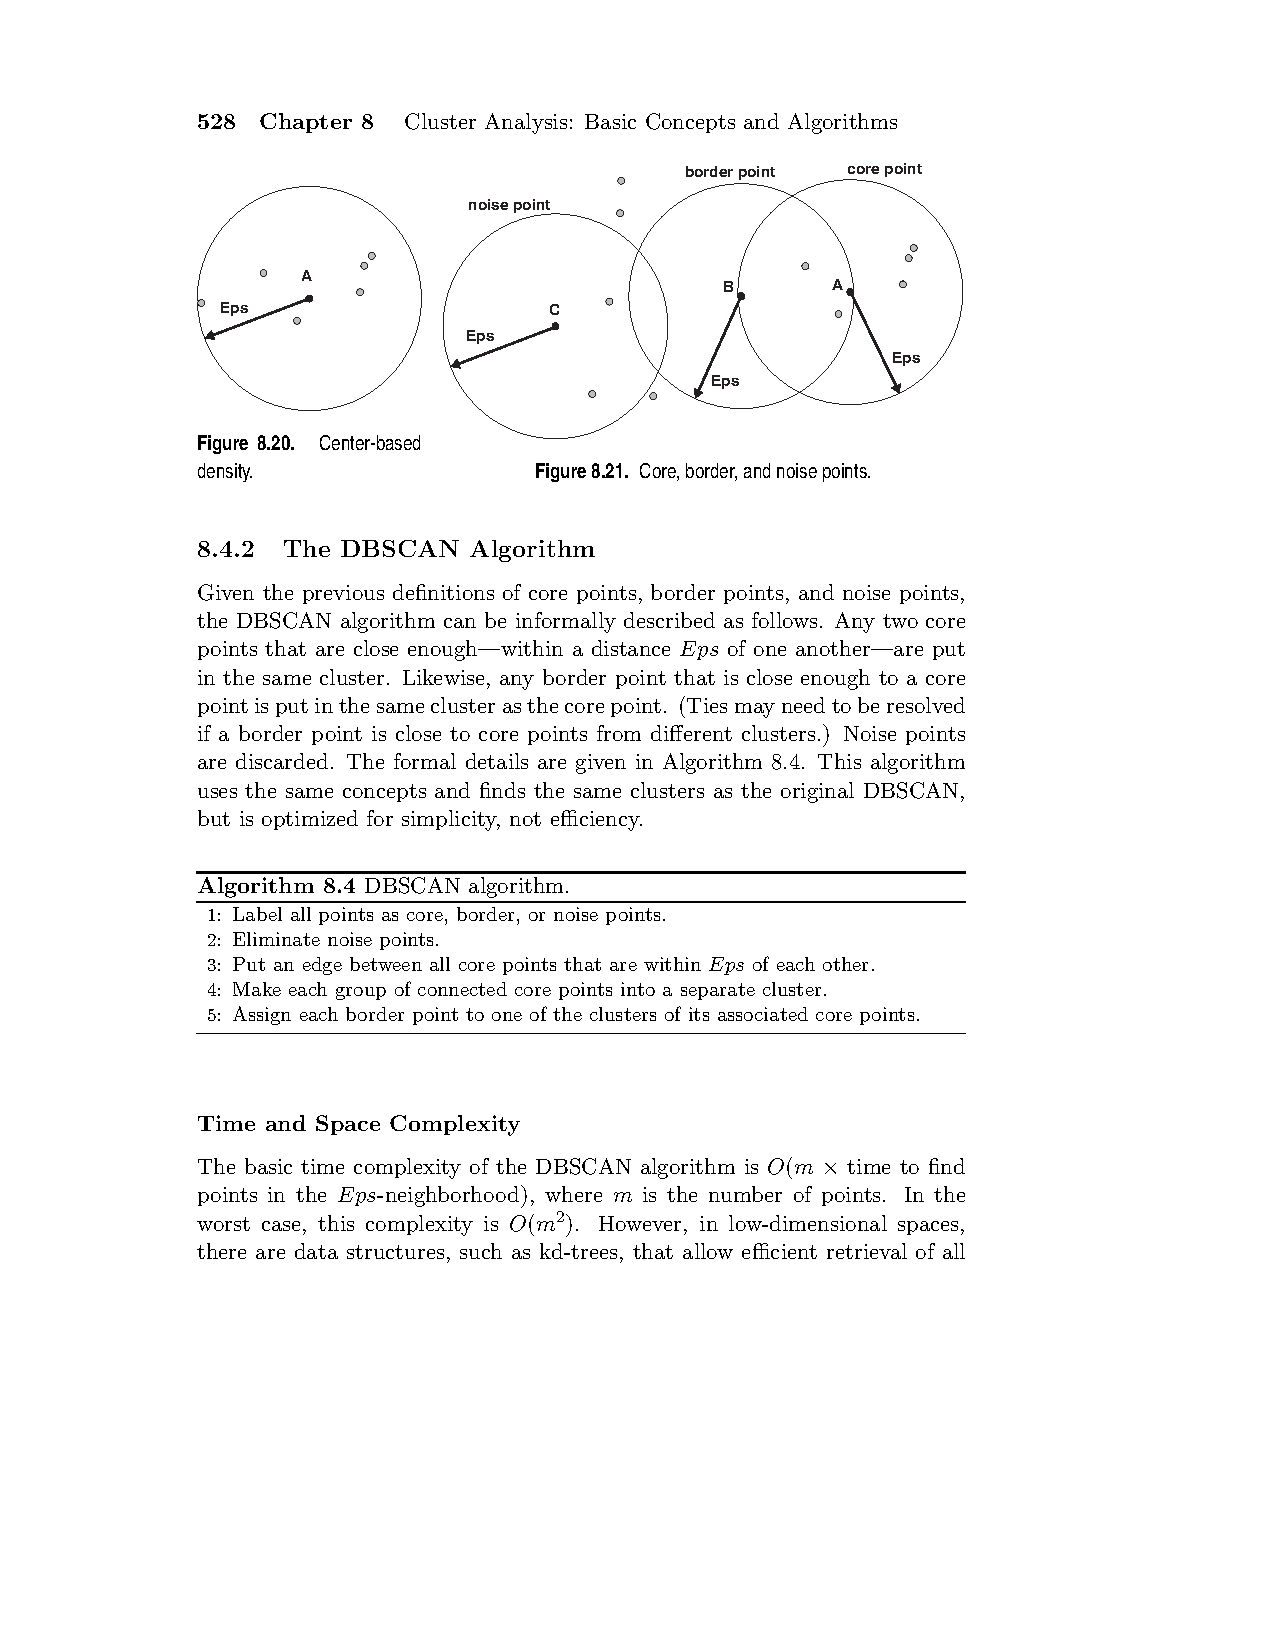
\includegraphics[trim= 3.1cm 20.61cm 5cm 2.5cm, clip=true]{graphics/DBSCAN_point_types}}
\caption{The three types of points in the clustering algorithm DBSCAN. Taken from \cite[page 528]{pang2006introduction}.}
\label{dbscan_point_types}
\end{figure}

A visual description can be seen on \Cref{dbscan_point_types}.
Given these definitions, the algorithm is described in \Cref{dbscan-algo}.

\begin{algorithm}
DBSCAN(D, eps, MinPts)\\
	C = 0\\
	\For {each unvisited point P in dataset D mark P as visited\\}
	{
		NeighborPts = regionQuery(P, eps)\\
		\eIf {sizeof(NeighborPts) < MinPts}{
			mark P as NOISE\\
		}
		{
			C = next cluster\\
			expandCluster(P, NeighborPts, C, eps, MinPts)
		}
	}
\caption{The DBSCAN clustering algorithm}\label{dbscan-algo}
\end{algorithm}

\begin{algorithm}
expandCluster(P, NeighborPts, C, eps, MinPts)\\
	add P to cluster C\\
	\For {each point Pn in NeighborPts\\}
	{
		\If{Pn is not visited\\}
		{
			mark Pn as visited\\
			NeighborPtsn = regionQuery(Pn, eps)\\
		}
		\If {sizeof(NeighborPtsn) >= MinPts\\}
		{
			NeighborPts = $ NeighborPts \cup NeighborPtsn $\\
			\If {Pn is not yet member of any cluster\\}
			{add Pn to cluster C\\}
		}
	}
\end{algorithm}%(Pn) is used instead of (p') in source (wiki).

\begin{algorithm}
regionQuery(P, eps)\\
	\Return {all points within the eps-neighborhood of P (including P)\\}
\end{algorithm}

\subsection{Summary} Of the three presented algorithms only the DBSCAN algorithm fits our need for a exclusive, partial and density based clustering algorithm.
We therefore use this algorithm to detect clusters in our data for use as the hotspots in our model.
The hierarchical need is covered by saving the clusters in a tree data structure\footnote{This was not implemented, see \Cref{ref:ods}.}.

\chapter{Web Service}
As we have very little knowledge of our target group\alexander{\mikael{What is our target group?}Developers with connections to city bikes?}, we would want our system to be as available as possible.
One way to do this, is to implement it on a multitude of platforms (e.g. PC, Android devices, iOS devices).
However, this would require massive work, as all these platforms are different and would therefore require different implementations.
Additionally, it would not be very flexible, as new platforms and devices are introduced on the market, requiring even further implementation.

Another way to make the system available, but without making it platform-dependent, would be to create a common web service that provides the most significant functionality of the system.

This section will shortly describe the possibilities when designing a web service, arguing why a RESTful web service is the correct choice for our system.

\subsection{Choosing an architecture}
When designing a web service, there are two overall architectural styles; REST (Representational State Transfter) and RPC (Remote Procedural Call).\cite{restful_web_services}
What we want to do is expose our resource state (part of our server state, e.g. bikes with their current locations).
As a RPC-style web service is by definition procedure-oriented, and what we want to do is expose resources, REST is the natural choice.

The following section will describe RESTful web services (specifically Resource-Oriented Architecture), based on \citet{restful_web_services}, \citet{fielding_dissertation}, and HTTP/1.1 Specification\cite{http_specification}.

\subsubsection{Representational State Transfer}
REST is an architectural style, which provides design criteria for network-based software architectures.
Web services adhering to these design criteria are referred to as RESTful web services.
These criteria were defined in \citet{fielding_dissertation}.
As REST is only an architectural style, making it possible to implement various correct architectures, we will be following one specific architecture implementation: Resource-Oriented Architecture (ROA) as described in \citet{restful_web_services}.

\subsubsection{Resource-Oriented Architecture}
ROA is an architecture, upholding the REST design criteria.
This is done by organizing and accessing resources in a standardized manner, and by following and taking full advantage of the HTTP/1.1 specification.

In order to ensure that a ROA implementation will comply with the REST design criteria, it will have to adhere to the four concepts: \textit{resources, URIs, representing resources, linking resources}, along with the four properties: \textit{addressability, statelessness, connectedness, uniform interface}.\cite[Chapter 4]{restful_web_services}

\paragraph{Resources} are a subset of the resource state.
A single resource is an entity important enough to be a thing in itself.

Each resource should have at least one \textit{URI} (Unique Resource Identifier).
URIs ensure that each resource can be uniquely identified, directly handling the \textit{addressability} property.

\subparagraph{Representations} of resources depends on the desired use.
A representation of a specific resource is a collection of any useful information about that resource's state, defined by properties and sub-resources.

\paragraph{Connectedness and linking resources} are highly dependent on URIs.
As each resource is uniquely identified, any resource containing sub-resources or needing to refer to other resources, can do so by linking to its URI. 

\paragraph{Statelessness} is handled by providing, if any, state-relevant parameters on each request.
This makes the server independent of clients and previous requests, as it is up to each individual client to handle its own application state (not to be confused with the server's resource state) and providing it when needed.

\paragraph{Uniform interface} is where the HTTP/1.1 specifications come in.
By taking advantage of the HTTP methods GET, POST, PUT, DELETE, HEAD, and OPTIONS, every resource is handled the same way.
POST, GET, PUT, and DELETE correspond to the Create, Read, Update, Delete (CRUD) operations.
HEAD is for retrieving the resource's meta-data, without the actual representation.
OPTIONS is for seeing allowed methods for a given resource (additionally, by providing the Authorization header, actions can be restricted based on client permissions).

Any feedback needed to be given to clients from the server is handled through HTTP status codes (e.g. '200 OK', '404 Not Found').


\chapter{Design and Implementation}
This chapter contains a description of the systems architecture and an overview of the data flow.
For the architecture each component will be described containing a full description of the system.
\section{Overview}
To ease the maintenance and ensure scalability, we have structured the project in an architecture which supports scalability.
The architecture consists of four macro components and a database, as can be seen in \cref{fig:architecture}. The macro components are: Shared, Location Service, Model Agent, and Web Service.\alexander{Maybe change the component name of `Model Updater' so it does not conflict with the layer name? \alexander{Changed name of component to `Model Agent'.}}

\begin{figure}[H]
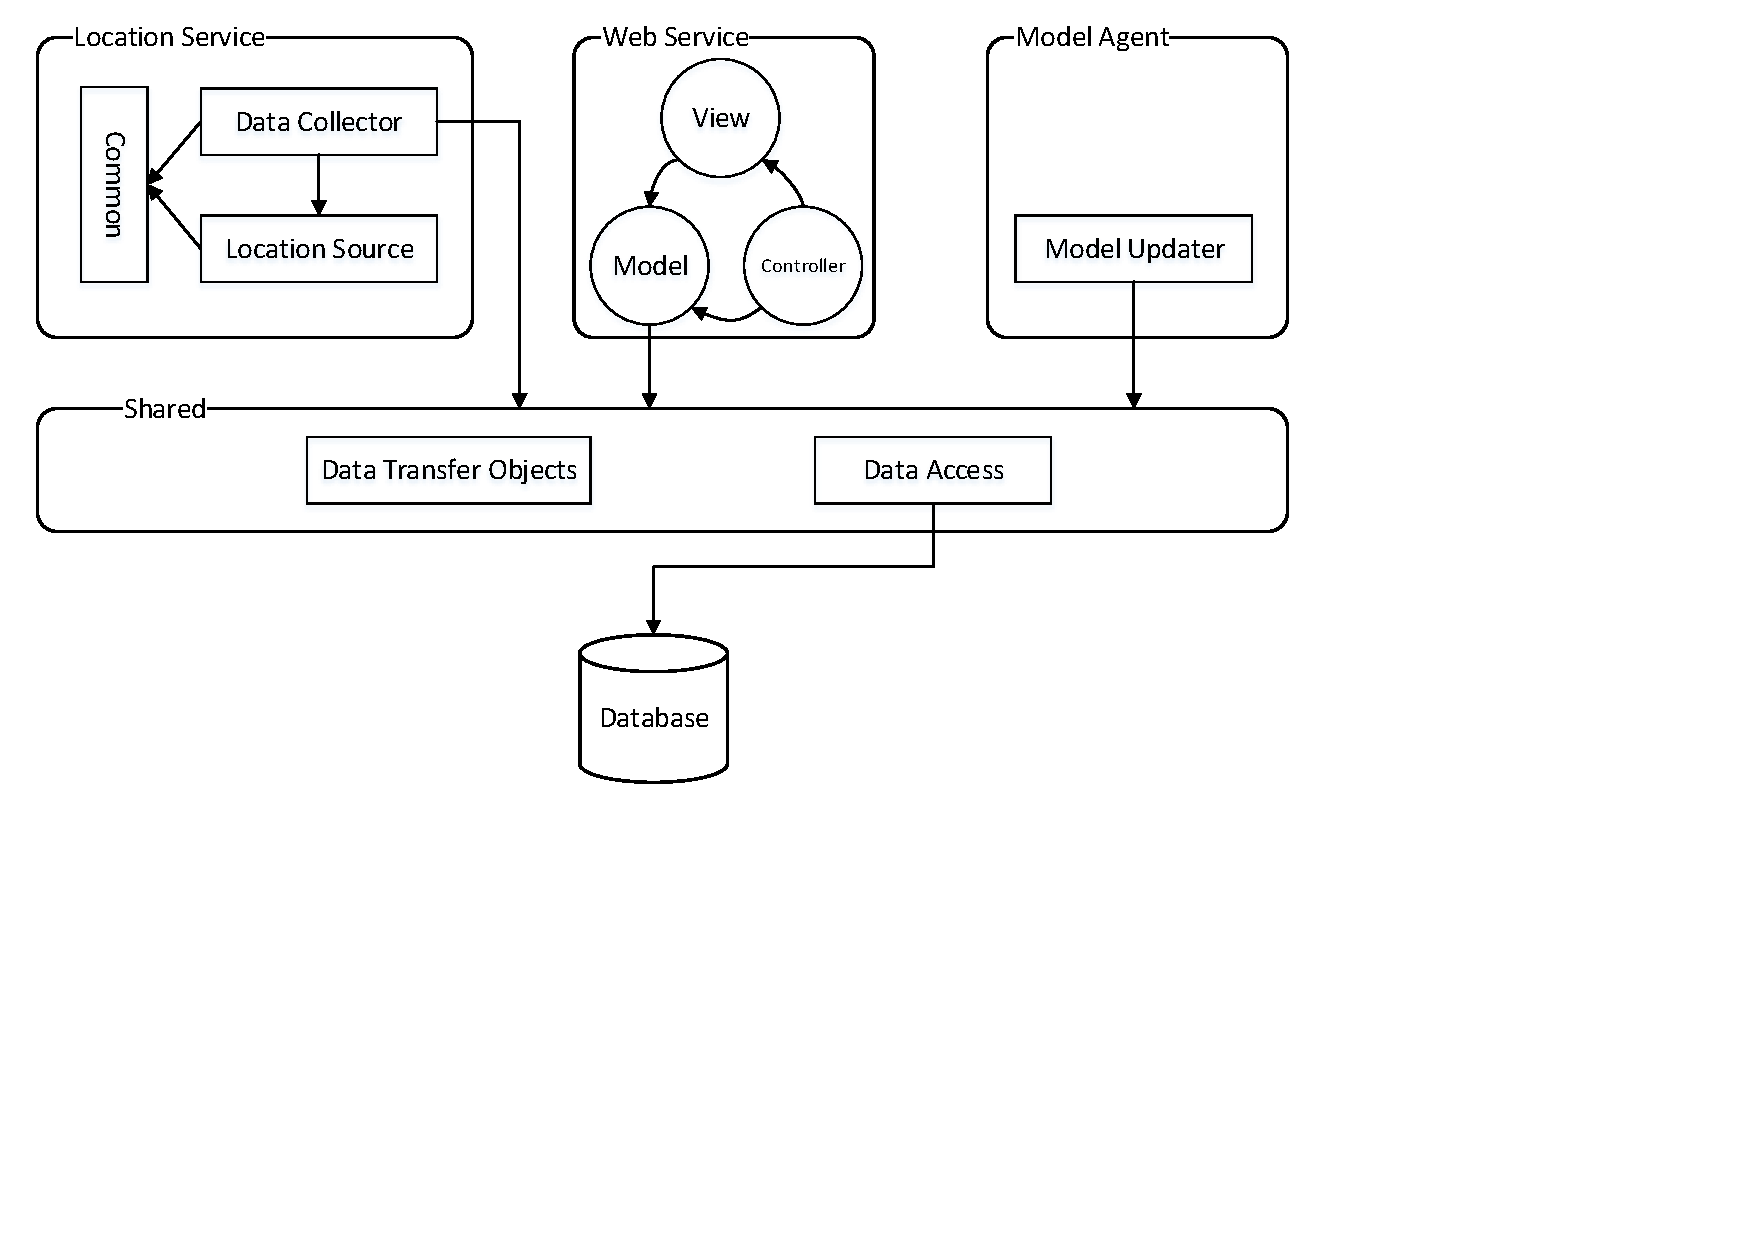
\includegraphics[width=\textwidth, trim={2cm 1cm 6cm 0}]{systemArchitecture.pdf}
\caption{The architecture of the system}
\label{fig:architecture}
\end{figure}

\subsection{Database} The database used is a MySQL database, and is where all our data is stored.
The design of the database can be found in \cref{database_design}


\subsection{Shared}\texttt{Shared} is the macro component containing the \texttt{Data Access} layer and the \texttt{Data Transfer Object} layer.
The macro component's task is to provide extended capabilities to all other macro components.

\paragraph{The Data Access layer} All SQL statements and communication with the database are encapsulated here providing the upper layers methods to communicate with the database.

\paragraph{The Data Transfer Object layer} contains all the shared data types and their attributes, making it possible for all the macro components to treat the data uniformly.


\subsection{Location Service} processes and stores location data directly from a data source. 
The \texttt{Location Service} consists of a \texttt{Location Source} which provides data points the \texttt{Data Collector}.

\paragraph{The Location Source layer} fetched data from the data source then adapts and casts the data to the appropriate data type in the \texttt{Common} layer.
It is structured so the \texttt{Location Source} layer can easily be replaced with another source of data.

\paragraph{The Data Collector layer} gathers the data from the \texttt{Location Source} layer and processes it. 
The data is then stored through the \texttt{Data Access} layer.


\subsection{Model Agent\footnote{An agent is defined as a program that invoke a given task, when a condition is satisfied, then returning to a sleeping state, until the condition is satisfied again.\cite{definitionagent}}}\texttt{Model Agent} is the macro component containing the \texttt{Model Updater} layer.
The macro component's task is to generate and update the model in the system. 

\paragraph{The Model Updater layer} handles the calculation and generation of the models.
The generation of the model works as follows:
Clusters are created based on the GPS data in the database
The convex hull of the clusters is calculated and saved as the hotspots of the model.
Markov chains are now created with these clusters as states.

\subsection{Web Service}\label{arch:webservice}
\texttt{Web Service} is the macro component containing the \texttt{Model}, \texttt{View}, and \texttt{Controller}.
The task of the macro component is to provide a web service for users to interact with the system.

\paragraph{The Model} manages the application domain and handles data and actions possible for each data type.

\paragraph{The View} manages the display of the \texttt{Model}.

\paragraph{The Controller} handles the user interaction. Based on the user request, the \texttt{Controller} sends commands to the \texttt{Model} and \texttt{View}.
\section{Scalability}
Scalability is an important factor when designing a web service. In this project the main potential growing assets are users and bikes.

Users are important to take into account, since we have high uncertainty in regards to the number of users, which could lead to performance issues if not addressed.

Additionally, the number of bikes should be increasable without causing problems in the system. If not addressed, it could lead to storage issues due to the increase in GPS data and increase in the time required to build the models.
A high number of resulting hotspots will also result in slower response times for the users due to the increased complexity of the predictions.

The easiest way to address these issues is to scale out (adding new hardware) or scale up (enhance existing hardware). \cite{michael2007scale}

\paragraph{The system} is scalable due to the way the macro components are divided. By dividing the system into macro components with their own tasks, it would be easy to add more hardware. It should further be easy to implement additional functionality due to the \texttt{Shared} macro component.

\bruno{THis shouldprobably be elaborated maybe with some examples.}
\section{Database Design}
\stefan{This section may be redundant, and an entry in appendix may be better.}
To store the data we use a MySQL database.
The following will describe the database design and the choices involved.

When data is collected and stored, it is stored in the \texttt{GPS\_data} table.
This table contains all information necessary for storing a GPS point as well as the field "hasNotMoved" which is used to indicate whether the bike is standing still or if it has moved since the point was insertet into the database.
This has been done in order to reduce redundant data in the database.
The GPS\_data table can be seen in \cref{tbl_gpsdata}

\begin{lstlisting}[caption=Table for GPS\_data, label=tbl_gpsdata, language=SQL]
CREATE TABLE gps_data (
	id INT UNSIGNED NOT NULL AUTO_INCREMENT UNIQUE PRIMARY KEY,
	bikeId INT UNSIGNED NOT NULL,
	latitude DECIMAL(10,8) NOT NULL,
	longitude DECIMAL(11,8) NOT NULL,
	accuracy TINYINT UNSIGNED NOT NULL,
	queried DATETIME NOT NULL,
	hasNotMoved BOOL NOT NULL DEFAULT FALSE
);
\end{lstlisting}

In order to query information about a single bike, and to keep track of the bikes currently available in the system.
The table for this is very simple and can be seen in \cref{tbl_bikes}

\begin{lstlisting}[caption=Table for bikes, label=tbl_bikes]
CREATE TABLE bikes (
 id INT UNSIGNED NOT NULL UNIQUE PRIMARY KEY
);

\end{lstlisting}

The hotspots created by the DBSCAN algorithm are also saved in the database.
A hotspot is described by a convex hull of the points that describe the area of the hotspot.
This convex hull is saved as binary data (a blob).

\begin{lstlisting}[caption=Table for hotspots, label=tbl]
CREATE TABLE hotspots (
	id INT UNSIGNED NOT NULL AUTO_INCREMENT UNIQUE PRIMARY KEY,
	convex_hull BLOB NOT NULL
);
\end{lstlisting}
\section{Web Service API}\label{design:web_service}
The web service API was implemented using ASP.NET Web API 2.3\cite{aspnet_webapi}.
ASP.NET Web API uses ASP.NET MVC\cite{aspnet_mvc}, with the use of \texttt{ApiController}, instead of the regular \texttt{Controller}.
In the architecture, the web service is defined as a component of its own (see \cref{arch:webservice}).

\subsection{Resource Oriented Architecture}
Resource Oriented Architecture criteria, as described in \cref{webservice:roa}, set the ground rules for designing the API.
These criteria are therefore upheld by the API.

\subsubsection{Resources}\label{webservice:resources}
This section contains the resources designed and implemented in the web service.
Resources in the implementation are objects, containing named properties and sub-resources.
Sub-resources are represented as simple objects, containing only its relative URL.
Each resource is described following this structure:
\begin{itemize}
\item \textbf{URL} the URL of the resource
\item \textbf{Properties} a property which can be accessed from this resource
\item \textbf{Resources} the resource(s) which can be accessed from this resource
\item \textbf{Methods} HTTP methods which can be used on that resource
\item \textbf{Responses} HTTP status codes which could be returned by this resource
\end{itemize}

\subsubsection*{The resources implemented:}
\bruno{Skal de i appendix eller skal det sættes op på en anden måde?}

% Command for displaying url, properties, and sub-resource of each resource
\newcommand{\resource}[5]{\begin{description}
\item[URL:]{\texttt{#1}}
\item[Properties:]{\texttt{#2}}
\item[Resources:]{\texttt{#3}}
\item[Methods:]{\texttt{#4}}
\item[Responses:]{\texttt{#5}}
\end{description}}

\resource{/}{version}{availablebikes, hotspots, bikes}{GET}{200 OK}
The root path serves as the entry point for the API.
It has a single property; version, to be used for asserting that the API has changes that implementations should react to.
More importantly, it contains a sub-resource for each main resource.

\noindent\hrulefill

\resource{/availablebikes}{count}{List of availablebikes}{GET}{200 OK}
This resource contains a list of all \texttt{availablebike} resources, along with a count of how many there are.

\noindent\hrulefill

\resource{/availablebikes/\{bikeId\}}{latitude, longitude}{}{GET}{200 OK, 404 Not Found}
This is the actual \texttt{availablebike} resource.
In case a client tries to request a bike that is not available, it will be met with a \texttt{404 Not Found} response.

\noindent\hrulefill

\resource{/hotspots}{hotspots}{}{GET}{200 OK}

This ressource returns all the hotspots in the system.

\noindent\hrulefill

\resource{/predictions}{}{}{GET}{200 OK}
This is the prediction resource.
When a client wants to know when a bike arrives at a hotspot this ressource can be used.

\subsection{MVC} 
MVC or Model-View-Controller\cite{aspmvc} is used to separate responsibility of an application into three parts, the model, the view, and the controller.
The pattern can be seen in \Cref{mvcdiagram}.

\begin{figure}[h]
\begin{center}
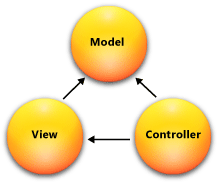
\includegraphics[width=\textwidth, trim={-4cm 11cm 5cm 1cm}]{mvc.pdf}
\caption{The MVC design pattern.}
\label{mvcdiagram}
\end{center}
\end{figure}

\paragraph{Model} contains the model of the application domain and takes care of fetching data and making it available through the model.

In the case of our web service, the model is making resources available for the view.

\paragraph{View} displays the model to the user.
In our case the view is the serialized resource representation, that the user obtains by performing requests against the API.
Per default, this is \texttt{text/xml}, however, by adding the \texttt{Accept} header, this can be set to \texttt{application/json} \cite[Section 14]{http_specification}.

\paragraph{Controller} handles the interaction with users.
Based on user input, the controller works on the model and selects what the view needs to be used for displaying the data.

The routing to controllers is handled by the attributes \texttt{[RoutePrefix]} and \texttt{[Route]}.
In order to handle the different HTTP methods, controller methods are also annotated with an appropriate \texttt{[Http\{Method\}]} attribute (e.g. \texttt{[HttpGet]}) \cite{asp_routing}.


\section{The Data Loading component}
The data loading component has the responsibility for fetching GPS points and processing them before inserting them into the database.
The component consists of a \texttt{Data Collector}, a \texttt{Location Source}, and a \texttt{Common} layer that contains an interface and data transfer objects.

The parts of this component will be described in this section.
\begin{figure}[h]
\centering
\begin{tikzpicture}[
path/.style={
	->,
	>=stealth
},
every node/.style={font=\sffamily,minimum height=1cm}]

\node[draw,minimum width=4cm,xshift=0.5cm](datacollector){Data Collector};

\node[draw,below=of datacollector](locationsource){Location source};

\node[draw,right=of datacollector, rotate=90,anchor=south,xshift=-0.9cm,yshift=-0.5cm, minimum width=2.5cm](common){Common};

\node[above=of datacollector, yshift=-1.2cm,xshift=-0.9cm](dataloading){Data loading};

\draw ($ (dataloading.north west) + (-0.3,0.3) $) rectangle ($ (common.south west)+(0.3,-0.7) $);

\draw[path] (datacollector.south) -- (locationsource.north);
\end{tikzpicture}
\caption{The Data Loading Component. The full diagram can be seen on \cref{arch}}
\label{dataloadingcomponent}
\end{figure}
\alexander{Shouldn't there be arrows from `Data Collector' and `Location Source' to `Common'?}

\subsection{Common}
The \texttt{Data Loading} component contains interfaces and data transfer objects for the \texttt{Data Loading} component.

The \lstinline!GPSInput! class works as a data transfer object for \lstinline!GPSData! in the \texttt{Model} layer of the \texttt{Business Logic} component.

The \lstinline!IDataSource! interface defines the behaviour of a data source in the system enabling the source to be changed.
The interface can be seen in \cref{idatasourcecode}.

\begin{lstlisting}[language=C,caption=The IDataSource interface,label=idatasourcecode]
public interface IDataSource
{
	GPSInput GetData();
}
\end{lstlisting}

The \lstinline!GetData();! method returns the oldest \lstinline!GPSInput! available if any is available.
If no \lstinline!GPSInput! is available it returns null.

\subsection{Data Collector}
The \texttt{Data Loader} works as an independent program that continuously asks the \lstinline!Location Source! for new \lstinline!GPSInput!.
The \lstinline!Location Source! is an implementation of the \lstinline!IDataSource! and the \texttt{Data Loader} can therefore use any source that implements this interface.

\subsection{Location Source}\label{design:location_source}
The \texttt{Location Source} contains implementations of the \lstinline!IDataSource! and will therefore contain an implementation of the simulation of bikes.
In the real system an implementation will be made where the data is fetched from the GPS trackers on the bikes instead.

The implementation of the bike simulation will be described in \cref{design:datasimulation}.
 
\section{Shared}
As mentioned this component contains two layers, the \texttt{Data Access Layer}(DAL) and the \texttt{Data Transfer Objects}(DTO) layer.
This components responsibility is to share data to other components by using the shared DTO's.
This component is used by the following layers; \texttt{Data Collector}, \texttt{Model} and \texttt{Model Updater}.

\paragraph{The DAL} contains the methods for reading and writing to the chosen database.
The DAL is used by layers to update and retrieve data from the database.

\paragraph{The DTO} layer contains objects used across the architecture so it is easier to move data around using the DAL.
\section{Data Flow}
This section is about the data flow. More precisely how the data that is received from the GPS receiver is send to the database and what it is used for.
A diagram of the flow can be seen below on \cref{fig:dataFlowDiagram}.
The diagram is explained in the following.

\begin{figure}[H]
\includegraphics[width=\textwidth, trim={0 25cm 8cm 0}]{dataflowdiagram.pdf}
\caption{The data flow diagram of our solution}
\label{fig:dataFlowDiagram}
\end{figure}
\pagebreak 

\paragraph{Database}
The database is explained \cref{} \bruno{ref når det er skrevet.}

\paragraph{From raw location data to \texttt{GPS data}}
Each bike is equipped with a GPS receiver which uses this to calculate its location.
The data is then send containing the location and a number indicating the accuracy of the location.
The data received is read and transformed to an object.
The object is inserted into the database.

\paragraph{From \texttt{GPS data} to Hotpots}
The \texttt{GPS data} are available from the database and is used by the clustering algorithm DBSCAN(\cref{clustering:DBSCAN}) to find all clusters.
By using convex hull (\cref{} \bruno{ref til convex hull - hvis vi skriver om det ellers bare en ekstern ref}) on each cluster the amount of \texttt{GPS data} is greatly minimized and is saved as a \texttt{Hotspot}.
The \texttt{Hotspot}'s are then saved to the database.

\paragraph{From Hotspots to Markov Chain}
This is building the Markov Chain(\cref{markov}) from the routes and \texttt{Hotspot}'s stored in the database.
The Markov Chain is then saved in the database.
In order to test how well our system works we have chosen to perform an integration test of some of the integral parts of the system, the clustering and the predictions.
Because we do not have access to bikes with GPS receivers mounted we have created a simulation that will mimic the real world as close as possible.
This chapter will first explain how we have simulated the real system and will afterwards present the performed integration test.

\section{Data Input Simulation}\label{design:datasimulation}
In the running system, locations will be retrieved from a GPS reciever attached on the bikes.
Because we do not have bikes with GPS receivers at our disposal, we need to create a realistic simulation of the behaviour of the system.

\subsection{Point generation}
Because we do not have access to a running system with X amount of bikes sending locations, we have created a simulation of the real system.
This system uses Google Directions to create pseudo-realistic routes and returns the locations at an interval.
In order to generate points that are as realistic as possible we have used the following approach for generating GPS points:

\begin{description}
\item[Create routes with Google directions] The Google Directions API \cite{gdirections} has been used to create realistic looking bike routes.
The API has a variety of settings to restrict the results, including a setting to only get bike routes.
\alexander{Beskriv hvad vi har gjort med Googles API og fjern eksempel fra appendix.}
The result can be either XML or JSON and contains the route structured by a number of ``steps''.\footnote{Actually a route contains a number of  ``legs'' which contains a number ``steps''. 
A leg is a part of a journey and a new leg will be created when changing means of transport or at waypoints.
For our purposes all routes will always contain only one leg.}
Steps are the points where the route changes direction and are the points that would be used to print a directions instruction for the route.
The result of a query to the Google directions API is a route that can be used by a human to find his way to his destination.

\item[Generate intervals] The route generated by Google directions only has points where the route changes direction.
In order to make the generated routes fit with the data generated by a GPS receiver, some points are added between two consecutive points, so that the generated GPS points are spaced out at a interval.
\alexander{Beskriv hvordan vi rigtig har gjort. Ved at bruge intervaller af 5 min.}
The generated GPS points are also delayed randomly.
Lost GPS points are not taken into account.
\alexander{Begrundelse af hvorfor punkter er delayed. Punkter er ikke delayed randomly, men det er random om de er delayed.}

\item[Perturb points to simulate precision] As one of our assumptions about GPS receivers are that they are not 100 \% accurate, and they will therefore not provide accurate locations, we will have to take this into account when generating points with Google Directions.
To simulate this inaccuracy, every generated point will be perturbed by a random value, corresponding to an expected inaccuracy.
This expected inaccuracy should correspond to GPS inaccuracy, which is up to 15 m according to \citet{garmingps}.
\end{description}

\section{Model Updater Component}
The \texttt{Model Updater} component contains the \lstinline!Model Updater Agent!.\alexander{Find source and description of the term Agent.}
It has access to the \texttt{Shared} component for database access and data types.

\paragraph{The Model Updater Agent} is an independent program which updates the Markov Chain. First the agent fetches the data types hotspots and routes, defined in the DTO layer, through the DAL. Then it calculates the Markov Chain and lastly it puts the new Markov Chain into the database through the DAL.
\alexander{Define `route' as all connected GPSPoints for a single bike.}


\chapter{Test}
\section{Integration test}

In order to test that our components interact together according to the specifications, we have chosen to perform integration testing of the system.

Integration testing has the purpose of testing that two units work together. 
Traditionally, integration testing is done by integrating two modules at a time, either from the top of the dependency tree or from the bottom.
There exists a variant, in which the whole system is tested together, instead of pair-wise, called big bang integration testing.
We have chosen to perform our test with this method, due to time limitations \cite{inttest}.

\subsection{Test setup}
The purpose of the tests we have designed is to check if the system can produce sensible predictions for the bikes in the system.

\stefan{coupling with problem statement}

In order to generate test data, we have created a method for simulating real world data. 
The simulator gets a list of destinations (in the form of addresses) as input, making it possible to adjust the probability of the system, by deliberately choosing certain destinations.
This makes it possible to create a data set, where it is possible to predict the expected result.

\paragraph{What to test}
We want to test the following parts of our system:

\begin{itemize}
\item Finding hotspots
\item Predictions
\end{itemize}

\subsection{Finding hotspots}
The system relies on the clusters to be indicative of how the bikes are used. 
All predictions uses the hotspots as a basis and misplaced hotspots can therefore skew the results, degrading the precision of the predictions.
We therefore want to test if the hotspots generated are as they are expected.

\paragraph{Test data and cases}
For this test, a data set has been created.
It consists of five addresses and their corresponding GPS coordinates.
We will then compute the hotspots based on this data and compare the center of these hotspots with the addresses they are generated from.
Because the addresses are the only place where the bikes stand still, there should only be clusters by the addresses.
This will give an indication of how well our hotspots are created.

Three of the points are well separated, in order to test the general cluster creation.
The last two points are placed one street from each other, in order to test how the clustering handles close points.
\stefan{ikke sikker på om den del giver mening}

\subsection{Predictions}
The users rely on the predictions of bikes to be somewhat telling of how the bikes move around in the city.
It is therefore important to test how well the predictions work.

\paragraph{Test data} To test this we create a number of controlled data sets.
The data sets are controlled by assigning probabilities of choosing the destinations. 
We then know where to expect the probabilities to be high.

\paragraph{Test cases}
The obvious test case is when the generated data has equal probability of choosing every destination. 
In this case we would expect the probabilities of a bike arriving at every destination to be the same.

Another test case is to weigh one destination higher than the others.
In this case we would expect the probability of a bike arriving at this particular destination to be higher than all the other probabilities.

\chapter{Other}
\subsection{MVC} 
MVC or Model-View-Controller\cite{aspmvc} is used to separate responsibility of an application into three parts, the model, the view, and the controller.
The pattern can be seen in \Cref{mvcdiagram}.

\begin{figure}[h]
\begin{center}
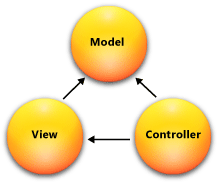
\includegraphics[width=\textwidth, trim={-4cm 11cm 5cm 1cm}]{mvc.pdf}
\caption{The MVC design pattern.}
\label{mvcdiagram}
\end{center}
\end{figure}

\paragraph{Model} contains the model of the application domain and takes care of fetching data and making it available through the model.

In the case of our web service, the model is making resources available for the view.

\paragraph{View} displays the model to the user.
In our case the view is the serialized resource representation, that the user obtains by performing requests against the API.
Per default, this is \texttt{text/xml}, however, by adding the \texttt{Accept} header, this can be set to \texttt{application/json} \cite[Section 14]{http_specification}.

\paragraph{Controller} handles the interaction with users.
Based on user input, the controller works on the model and selects what the view needs to be used for displaying the data.

The routing to controllers is handled by the attributes \texttt{[RoutePrefix]} and \texttt{[Route]}.
In order to handle the different HTTP methods, controller methods are also annotated with an appropriate \texttt{[Http\{Method\}]} attribute (e.g. \texttt{[HttpGet]}) \cite{asp_routing}.


\appendix
\chapter{Google Directions XML output}\label{gdir}

The output for the http request

\begin{lstlisting}
https://maps.googleapis.com/maps/api/directions/xml?origin=Chicago,IL&destination=Chicago,IL
\end{lstlisting}


\begin{lstlisting}
<?xml version="1.0" encoding="UTF-8"?>
<DirectionsResponse>
 <status>OK</status>
 <route>
  <summary>S Federal St</summary>
  <leg>
   <step>
    <travel_mode>DRIVING</travel_mode>
    <start_location>
     <lat>41.8781139</lat>
     <lng>-87.6297872</lng>
    </start_location>
    <end_location>
     <lat>41.8781139</lat>
     <lng>-87.6297872</lng>
    </end_location>
    <polyline>
     <points>eir~FdezuO</points>
    </polyline>
    <duration>
     <value>0</value>
     <text>1 min.</text>
    </duration>
    <html_instructions>Tag </html_instructions>
    <distance>
     <value>0</value>
     <text>1 fod</text>
    </distance>
   </step>
   <duration>
    <value>0</value>
    <text>1 min.</text>
   </duration>
   <distance>
    <value>0</value>
    <text>1 fod</text>
   </distance>
   <start_location>
    <lat>41.8781139</lat>
    <lng>-87.6297872</lng>
   </start_location>
   <end_location>
    <lat>41.8781139</lat>
    <lng>-87.6297872</lng>
   </end_location>
   <start_address>Chicago, Illinois, USA</start_address>
   <end_address>Chicago, Illinois, USA</end_address>
  </leg>
  <copyrights>Kortdata 2014 Google</copyrights>
  <overview_polyline>
   <points>eir~FdezuO</points>
  </overview_polyline>
  <bounds>
   <southwest>
    <lat>41.8781139</lat>
    <lng>-87.6297872</lng>
   </southwest>
   <northeast>
    <lat>41.8781139</lat>
    <lng>-87.6297872</lng>
   </northeast>
  </bounds>
 </route>
</DirectionsResponse>

\end{lstlisting}
\chapter{Interview 10-10-2014}\label{interviewReferat}
\section{Interviewees}
\begin{itemize}
\item Brian Høj - Responsible for \citybike.
\item Jesper - Employed with \citybike.
\item Anne Mette - Part of launching the ACHIMEDES project.
\end{itemize}
\section{Interview Summary (in Danish):}
\paragraph{- Hvilket overblik har I over cyklerne? lokation, forbrug, antal, osv. Hvordan finder I ud af om der skal flere cykler i brug, og hvor cyklerne skal placeres?}
Der er i øjeblikket ingen kontrol med cyklerne og dermed heller ingen  data omkring brugen
af cyklerne. Den eneste information er gehør, altså hvad de selv observerer ude i byen,
og de opringninger de modtager fra borgerne der melder en cykel forsvundet.

\paragraph{- Får I nogle klager? Hvis ja, hvad lyder klagerne på?}
De klager de oftest får er at der ikke er nok cykler tilgængelig. De observerer også selv
at der er helt tomme stationer.

\paragraph{- Har I nogle statistikker/data om systemet vi kan få adgang til?}
Der er ingen data overhovedet. Kun anelser om hvordan cyklerne bliver brugt. En af de interviewede
observerede at der holdt mange bycykler ved skoler og universiteter, hvilket de fortolker som om
at der er mange der bruger cyklerne som privatcykler.
Hvad de fandt interessant er at få mere data om brugen af cyklerne. Dette kunne fås v.h.a. GPS, ruter, strækning, stationer, tid, 
stilstand, samme bruger?

\paragraph{- Kan vi bruge det samme layout som http://www.aalborgbycyklen.dk m.h.t. Copyright?}
De mener at det er dem der ejer siden, og vil lige undersøge om ikke også de har rettighederne.

\paragraph{- Hvad er jeres egentlige behov? Hvilke mål har i med projektet og hvilke restriktioner er blevet påsat jer for at opnå disse mål?}
De er usikre på om det er turister eller borgere der er målgruppen for brugen af cyklerne, men de ligger vægt på at den ikke
bliver brugt som privatcykler. For eksempel hvis en person ønsker at bruge den resten af året ud.
Den større politiske opmærksomhed på bycykler sammen med tendensen til at der bliver afsat flere penge af til sådanne projekter
leder dem til at konkludere at det er et system der skal udvides på, og gøres mere moderne.

\paragraph{- Har i nogle udvidelser/videreudviklings planer til projektet?}
De er interesseret i at tracke cyklerne med GPS og indsamle data om cyklernes brug, men de har ikke nogle konkrete planer om hvad
der skal laves og hvordan man sikrer at GPS'en ikke bliver stjålet fra cyklen.

\paragraph{- Har i haft nogle tanker om reservering af bycyklerne?}
Der var ingen tanker i den retning med systemet, men idéen om at booke en cykel virkede interessant for dem. De var åbne overfor
muligheden, men kunne også ulemperne ved et sådant system, da det kan blive for restriktivt i forhold til brugeren.
For eksempel, hvad sker der hvis brugeren slet ikke dukker op til sin booking? Hvor længe i forvejen skal man kunne booke en cykel?
Hvornår må systemet konstatere at brugeren ikke dukker op?
De ser brugen af cyklerne som en spontan handling fra brugeren og måske ikke så meget planlagt.
 
\paragraph{- Har i lyst til at være vores kunde? Højst 3 møder mere i løbet af semester.}
Ja, de var villige til at lave en forsøgsperiode på en uge eller mere, hvor eksempelvis ti cykler blev udstyret med GPS, så man kunne
studere cyklernes færden.
Aftalen lyder, at vi tre grupper snakker sammen om vores videre arbejde og kontakt med dem som kunder.

\section{Interview Notes (in Danish):}

\begin{itemize}
\item Oprindeligt 200 cykler men kun 140 cykler ude nu. Resten er i depot.
\item Et privat firma der står for driften. En dyr ordning. Der mangles sponsor indtægter.
\item Ingen GPS på cyklerne. Simpelt system.
\item Har overvejet at se på noget mere avanceret. Måske nogle nye cykler? tænker de
Århus, har andre cykler hvor de ikke har problemer med sponsorer (store reklamer på hjulene). Færre driftsomkostninger
\item Der forsvinder ikke mange cykler. (ikke noget særligt)
\item Cyklerne samles ind i oktober. De finder allesammen, men de kan godt finde mærkelige steder. De kommer ud igen først i april.
\item De har problemer med at cyklerne ikke bliver fundet af sig selv men rapporteret forsvundet af brugerne.
\item De kunne godt tænke sig at have kontrol af cyklerne (med GPS har de overvejet)
\item De vil også gerne vide mønstrene af brug af cyklerne.
\item Der findes ingen data for brug af cyklerne. Det eneste der sker ved cyklerne er vedligeholdelse.
\item De vil gerne have turister til at bruge cyklerne
\item Målgruppen er: turist eller borger (ikke så meget hvem der er, men at den ikke bliver brugt som sin private cykel)
\item GPS ideen lyder spændende for dem.
\item De er bevidste om at det er en dårlig ordning.
\item De er interesseret i data og statistikker om hvordan det bliver brugt.
\item Booking er også interessant, men GPS delen er særlig interessant.
\item Hvor længe holder de stille? Hvor meget er de i brug?
\item Deres egne observationer er at der holder mange ved skoler og universiteter og kan måske konkludere ud fra det at de bliver brugt til privat brug.
\item De tror mere på de spontane brug af bycyklerne, og mener at det bliver meget restriktivt med booking.
\end{itemize}


\bibliography{bibliography}
\end{document}
